\documentclass[final,3p,11pt,pdflatex]{elsarticle}
\usepackage[utf8x]{inputenc}      % input font encoding
\usepackage{amsmath,amssymb}
\usepackage[T1]{fontenc}          % output font encoding
\usepackage{booktabs,tabularx}
\usepackage{rotating}             % for sidewaystable
\usepackage{xspace}
\usepackage[usenames]{xcolor}
\usepackage{tikz,tikz-uml}
\usepackage{listings}
\bibstyle{elsarticle-num}
% source code highlighting
\lstset{breaklines=true,
  breakatwhitespace=true,
  stepnumber=1,
  basicstyle=\ttfamily\footnotesize,
  commentstyle=\ttfamily\color{gray},
  prebreak={\textbackslash},
  breakindent=10pt,
  breakautoindent=false,
  showspaces=false,
  showstringspaces=false,
  frame=single,
  abovecaptionskip=0em,
  aboveskip=1.5em,
  belowcaptionskip=0.5em,
  belowskip=1em,
}
\usepackage[pdftitle={FlexibleSUSY --- A spectrum generator generator for supersymmetric models},
pdfauthor={Peter Athron,Jae-hyeon Park,Dominik Stockinger,Alexander Voigt},
pdfkeywords={FlexibleSUSY,supersymmetry,spectrum,generator,MSSM,NMSSM,E6SSM},
bookmarks=true, linktocpage]{hyperref}

%macros
\newcommand{\sarah}{SARAH\xspace}
\newcommand{\fs}{FlexibleSUSY\xspace}
\newcommand{\ESSM}{E$_6$SSM\xspace}
\newcommand{\code}[1]{\lstinline|#1|}  % inline source code
\newcommand{\textoverline}[1]{$\overline{\mbox{#1}}$}
\newcommand{\DRbar}{\textoverline{DR}\xspace}
\newcommand{\MSbar}{\textoverline{MS}\xspace}
\newcommand{\unit}[1]{\,\text{#1}}      % units
\newcommand{\userinput}{\text{<input>}}
\newcommand{\pole}{\text{pole}}
\newcommand{\Lagr}{\mathcal{L}}
\newcommand{\unity}{\mathbf{1}}
\newcommand{\figref}[1]{\figurename~\ref{#1}}
\newcommand{\secref}[1]{Sec.~\ref{#1}}
\newcommand{\tabref}[1]{\tablename~\ref{#1}}
\DeclareMathOperator{\diag}{diag}
\DeclareMathOperator{\sign}{sign}
\DeclareMathOperator{\re}{Re}
\DeclareMathOperator{\im}{Im}
\def\at{\alpha_t}
\def\ab{\alpha_b}
\def\as{\alpha_s}
\def\atau{\alpha_{\tau}}
\def\oat{O(\at)}
\def\oab{O(\ab)}
\def\oatau{O(\atau)}
\def\oatab{O(\at\ab)}
\def\oatas{O(\at\as)}
\def\oabas{O(\ab\as)}
\def\oatababq{O(\at\ab + \ab^2)}
\def\oatqatababq{O(\at^2 + \at\ab + \ab^2)}
\def\oatasatq{O(\at\as + \at^2)}
\def\oatasabas{O(\at\as +\ab\as)}
\def\oatasabasatq{O(\at\as + \at^2 +\ab\as)}
\def\oatq{O(\at^2)}
\def\oabq{O(\ab^2)}
\def\oatauq{O(\atau^2)}
\def\oabatau{O(\ab \atau)}
\def\oas{O(\as)}
\def\oatauqatab{O(\atau^2 +\ab \atau )}

\journal{Computer Physics Communications}
\begin{document}
\begin{frontmatter}

 \title{\Large\bf FlexibleSUSY --- A spectrum generator generator for supersymmetric models}

\author[adelaide]{Peter Athron}
\author[dresden]{Jae-hyeon Park}
\author[dresden]{Dominik St\"ockinger}
\author[dresden]{Alexander Voigt}
\address[adelaide]{ARC Centre of Excellence for Particle Physics at 
the Tera-scale, School of Chemistry and Physics, University of Adelaide, 
Adelaide SA 5005 Australia}
\address[dresden]{Institut f\"ur Kern- und Teilchenphysik,
TU Dresden, Zellescher Weg 19, 01069 Dresden, Germany}
   
  \begin{abstract}
   We introduce \fs, a MATHEMATICA package which generates a fast,
   precise C++ spectrum generator for any SUSY model specified by the
   user.  The generated code is designed with both speed and
   modularity in mind, making it easy to adapt and extend with new
   features. The user specifies the model supplying the
   superpotential, gauge structure and particle content in a \sarah
   model file and provides specific the boundary conditions in a
   separate \fs model file. \fs makes use of the existing \sarah
   package to obtain self energies, tadpole corrections,
   renormalisation group equations(RGEs) and tree level mass and
   electroweak symmetry breaking conditions for the specified model. These are
   translated into C++ code and combined  with numerical
   routines for solving the RGEs, EWSB conditions and simultaneously
   solving for the spectrum conssistent with user specified boundary
   conditions.  The modular structure of the generated code allows for
   individual components to be replaced with an alternative if
   available. \fs has been carefully designed to grow as
   alternative solvers and calculators are added.
  \end{abstract}

\begin{keyword}
sparticle, 
supersymmetry, 
Higgs
\PACS 12.60.Jv
\PACS 14.80.Ly
\end{keyword}
\end{frontmatter}

\section{Program Summary}
\noindent{\em Program title:} \fs\\ {\em Program obtainable from:}
         {\tt http://flexiblesusy.hepforge.org/}\\ {\em Distribution
           format:}\/ tar.gz\\ {\em Programming language:} {\tt
           C++}\\ {\em Computer:}\/ Personal computer\\ {\em Operating
           system:}\/ Tested on Linux 3.x\\ {\em Word size:}\/ 64
         bits\\ {\em External routines:}\/ SARAH 4.0.4, Boost library,
         Eigen, lapack\\ {\em
           Typical running time:}\/ 0.1-0.3 seconds per parameter
         point.\\ {\em Nature of problem:}\/ Determining the mass
         spectrum and mixings for any supersymmetric model. The
         generated code must find simultaneous solutions to
         constraints which are specified at two or more different
         renormalisation scales, which are connected by
         renormalisation group equations forming a large set of
         coupled differential equations. \\ {\em Solution method:}\/
         Nested iterative algorithm and numerical minimisation of the
         Higgs potential.  \\ {\em Restrictions:} The couplings must
         remain perturbative at all scales between the highest and
         lowest boundary condition.  \fs~ assumes that all couplings
         of the model are real (i.e.\ $CP-$conserving). Due to the
         modular nature of the generated code adaption and extension
         to overcome restrictions in scope is quite straight forward.





\newpage
\section{Introduction}
Supersymmetry(SUSY) provides the only non-trivial way to extend the
space-time symmetries of the Poincar\'e
group\cite{Coleman:1967ad,Haag:1974qh}, leading many to suspect that
SUSY may be realised in nature in some form. In particular
supersymmetric extensions of the standard model where SUSY is broken
at the TeV scale have been proposed to solve the hierarchy
problem\cite{Weinberg:1975gm, Weinberg:1979bn, Gildener:1976ai,
  Susskind:1978ms, 'tHooft:1980xb}, allow gauge coupling
unification\cite{Langacker:1990jh, Ellis:1990wk, Amaldi:1991cn,
  Langacker:1991an, Giunti:1991ta} and predict a dark matter candidate
which can fit the observed relic
density\cite{Goldberg:1983nd,Ellis:1983ew}.  Such models have also
been used for baryogenesis or leptogensis to solve the
matter-anti-matter asymmetry of the universe and have been considered
as the low energy effective models originating from string
theory.

Detailed phenomenological studies have been carried out for scenarios
within the minimal supersymmetric standard model (MSSM).  Such work
has been greatly aided by public spectrum generators for
MSSM\cite{Allanach:2001kg,Porod:2003um,Djouadi:2002ze,Baer:1993ae},
allowing fast and reliable exploration of the sparticle spectrum,
mixings and couplings, which can be obtained from particular choices
of breaking mechanism inspired boundary conditions and specified
parameters. Beyond the MSSM there are also two public spectrum
generators \cite{Ellwanger:2006rn,Allanach:2013kza} for the next to
minimal supersymmetric standard model (NMSSM) \cite{NMSSM}.

None of the fundamental motivations of supersymmetry require
minimality, and specific alternatives to (or extensions of) the MSSM
are, for example, motivated by the $\mu$-problem of the
MSSM \cite{Kim:1983dt}; explaining the family structure (see e.g,
\cite{King:2014nza}) or for successful baryogensis or leptogenesis
(see e.g,\cite{King:2008qb}). However constructing specialised tools
to study all relevant models would require an enormous amount of work.
So general tools which can automate this process and produce fast and
reliable programs can greatly enhance our ability to understand and
test non-minimal realisations of supersymmetry.

Recent experimental developments have also increased the relevancy of
such a tool. From the recent $7$ TeV and $8$ TeV runs at the Large
Hadron Collider (LHC) there have been two important developments.
First low energy signatures expected from such models, such as the
classic jets plus missing transverse energy signature, have not been
observed, substantially raising the lower limit on sparticle masses
(see e.g.~\cite{Aad:2013wta,Chatrchyan:2014lfa}). No other signature
of beyond the standard model(BSM) physics has been observed, leaving
the fundamental questions which motivated BSM physics
unanswered. Secondly ATLAS and CMS discovered\cite{ATLAS:2012ae,
  Chatrchyan:2012tx} a light Higgs of $125$ GeV, within the mass range
that could be accommodated in the MSSM but requiring stops which are
significantly heavier than both the direct collider limits and
indirect limits that appears in constrained models from the
significantly higher limits on first and second generation squarks.

These motivate both exploring non-minimal SUSY models which ameliorate
the naturalness problems by, for example, raising the tree level Higgs
mass, and models developed with a fresh perspective, based on other
considerations.  In both cases exploration of such models can be aided
if it is possible to quickly create a fast spectrum generator.
Currently there is only option for this, a SPheno-like FORTRAN code
which can be generated from
\sarah\cite{Staub:2010ty,Staub:2009bi,Staub:2010jh,Staub:2012pb,Staub:2013tta}.

\fs provides a much needed alternative to this with a structure which
has been freshly designed to accommodate as general range of models as
possible and to be easily adaptable to changing goals and new
ideas. \fs is a MATHEMATICA package which uses \sarah to create a
fast, modular C++ spectrum generator for a user specified SUSY model.
The generated code structure is designed to be as flexible as possible
to accommodate different types of extensions and due to it's modular
nature it is easy to modify, add new features and combine with other
programs.  The generated code has been extensively tested against well
known spectrum generators and as well providing a solution for new
SUSY models the generated MSSM and NMSSM codes offer a modern and fast
alternative to the existing public spectrum generators.

In section \ref{Sec:Program} we describe the program in more detail
and explain our design goals.  In section \ref{Sec:download}
information on how to download and compile the code may be found along
with details on how to get started quickly.  In section
\ref{Sec:modfile} we describe how the user can create a new
FlexibleSUSY model file. A detailed description of the structure and
features of the generated code is then given in section
\ref{Sec:SpecGenStruct}.  In section \ref{Sec:Flexible} we describe
the various ways the code can be modified both at the meta code level
by writing model files and at the C++ code level by modifying the code
or adding new modules. Finally in section \ref{Sec:comparison} we
describe detailed comparisons between our generated code and existing
public spectrum generators as well as against the SPheno-like FORTRAN
code which can be created using SARAH.


\section{Overview of the Program}
\label{Sec:Program}
\fs is a MATHEMATICA package designed to create a fast and easily
adaptable spectrum generator in C++ for any SUSY model and some
non-supersymmetric models.  The user specifies the model by giving the
superfield content, superpotential, gauge symmetries and mass mixings
in the \sarah model files, examples of which can be found in the
\code{Models} directory of \sarah and the \code{sarah} directory of
FlexibleSUSY.  The user then also specifies the boundary conditions on
the model parameters in a separate \code{FlexibleSUSY.m} file,
examples of which can be found in the \code{model_files} directory. A
detailed guide on how to write the FlexibleSUSY.m model is given in
section \ref{Sec:modfile}.

\fs makes use of the existing \sarah package
\cite{Staub:2010ty,Staub:2009bi,Staub:2010jh,Staub:2012pb,Staub:2013tta}
to obtain tree level expressions for the mass matrices and electroweak
symmetry breaking conditions, one-loop self energies, one-loop
tadpoles corrections and two-loop renormalisation group
equations(RGEs) for the model specified in the model files. Additional
corrections which have been calculated elsewhere, such as two-loop
corrections to the Higgs masses\footnote{By default FlexibleSUSY has
  two-loop corrections to the Higgs masses for the
  MSSM\cite{Degrassi:2001yf,Brignole:2001jy,Dedes:2002dy,Brignole:2002bz,Dedes:2003km}
  and NMSSM \cite{Degrassi:2009yq} in FORTRAN files supplied by Pietro
  Slavich. These are the same corrections which are implemented in
  many of the public spectrum generators.} may be added in file
specified by the user.

\fs then converts these algerbraic expressions from \sarah into C++
code using the C++11 standard. \fs uses some parts of
SOFTSUSY\cite{Allanach:2001kg}, the very fast Eigen library
\cite{eigen}, as well as the gnu scientific library and the boost
library to create numerical routines which solve the RGEs and EWSB
conditions.  The main solver routine of \fs then calls these routines
to find simultaneous solutions for the EWSB, low energy data, and
other, user supplied, boundary conditions (e.g.\ the usual mSUGRA
universality conditions) and calculates the mass spectrum.

The modular structure of the generated code allows for any individual
components to be replaced with an alternative if available.  Indeed
\fs has been intentionally designed to grow as alternative solvers and
calculators are added and a subsequent release with an alternative
lattice solver is already planned.  In addition if one already has an
existing code for some other purpose and simply wishes to improve upon
this by adding, e.g., new RGEs or self energies the modular framework
makes this straightforward by adding or interfacing with the
appropriate routine.

\subsection{Design goals}

FlexibleSUSY is designed with the following points in mind:

\paragraph{Speed}

Exploring the parameter space of supersymmetric models with a high
number of free parameters is quite time consuming.  Therefore \fs aims
to produce spectrum generators with a short run-time.  The two most
time consuming parts of a SUSY spectrum generator are usually the
calculation of the two-loop $\beta$-functions and the pole masses of
mixed particles:
%
\begin{itemize}
\item \emph{Calculation of the $\beta$-functions:} The RG solving
  algorithms usually need $O(10)$ iterations between the high and the
  low scale to find a set of parameters consistent will all boundary
  conditions with a $0.01\%$ precision goal.  During each iteration
  the Runge-Kutta algorithm needs to calculate all $\beta$-functions
  $O(50)$ times.  Most two-loop $\beta$-functions involve $O(50)$
  matrix multiplications and additions.  All together one arrives at
  $O(10^4)$ matrix operations.  To optimize these, \fs uses the fast
  linear algebra package \href{Eigen}{http://eigen.tuxfamily.org}.
  Eigen uses C++ expression templates to remove temporary objects and
  enable lazy evaluation of the expressions.  It supports explicite
  vectorization, and provides fixed-size matrices to avoid dynamic
  memory allocation.  All of these features in combination result in
  very fast code for the calculation of the $\beta$-functions in \fs.
%
\item \emph{Calculation of the pole masses:} The second most time
  consuming part is the precise calculation of the pole masses for
  mixed particles.  For each particle $\psi_k$ in a multiplet the full
  self-energy matrix $\Sigma^\psi_{ij}(p=m^\text{tree}_{\psi_k})$ has
  to be evaluated.  Each self-energy matrix entry again involves the
  calculation of $O(50)$ Feynman diagrams, each involving the
  calculation of vertices and a loop-function.  All in all, one
  arrives at $O(500)$ Feynman diagrams and $O(10^4)$ loop function
  evaluations.  To speed up the calculation of the pole masses \fs
  makes use of multi-threading, where each pole mass is calculated in
  a separate thread.  This allows the operating system to distribute
  these calculations among different CPU cores.  With this technique
  one can gain a speed-up of $20$--$30\%$.
\end{itemize}

\paragraph{Modularity}
The large variety of supersymmetric models makes it likely that the
user wants to modify the generated spectrum generator source code.
\fs uses C++ object orientation features to modularize the source code
in order to make it easy for the user to modify, reuse and extend the
spectrum generator.  An important application of this concept are the
boundary conditions: The RG solver provides a common \code{Constraint}
interface, see \figref{fig:schematic-two-scale-constraint-interface}.
%
\begin{figure}
  \centering
  \tikzumlset{fill class=white}
  \begin{tikzpicture}
    \umlclass[x=0, y=0]{RGFlow<Two\_scale>}{}{
      + solve()
    }
    \umlclass[x=6, y=0, type=abstract]{Constraint<Two\_scale>}{}{
      + \umlvirt{apply()}\\
      + \umlvirt{get\_scale() : double}
    }
    \umlclass[x=6, y=-3]{MyConstraint}{}{
      + apply()\\
      + get\_scale() : double
    }
    \umldep{RGFlow<Two\_scale>}{Constraint<Two\_scale>}
    \umlinherit{MyConstraint}{Constraint<Two\_scale>}
  \end{tikzpicture}
  \caption{Schematic two-scale constraint interface}
  \label{fig:schematic-two-scale-constraint-interface}
\end{figure}
%
To create a custom constraint \code{MyConstraint}, the user implements
the interface by inheriting from \code{Constraint} and writing the
\code{apply()} and \code{get_scale()} methods (see
\secref{sec:boundary-conditions} for more details).  The so created
constraint class can then be passed to the RG solver to impose the
user-defined boundary condition at the chosen scale.

\section{Download and compilation}
\label{Sec:download}

\subsection{Requirements}

\fs can be downloaded from \url{http://flexiblesusy.hepforge.org}.  To
create a custom spectrum generator the following requirements are
necessary:
%
\begin{itemize}
\item MATHEMATICA, version 7 or higher
\item SARAH, version 4.0.4 or higher \url{http://sarah.hepforge.org}
\item C++11 compatible compiler (g++ 4.4.7 or higher, clang++ 3.1 or
  higher, icpc 12.1 or higher)
\item FORTRAN compiler (gfortran, ifort etc.)
\item Eigen library, version 3.1 or higher
  \url{http://eigen.tuxfamily.org}
\item Boost library, version 1.36.0 or higher
  \url{http://www.boost.org}
\item GNU scientific library \url{http://www.gnu.org/software/gsl/}
\item lapack \url{http://www.netlib.org/lapack/}
\end{itemize}
%
Optional:
%
\begin{itemize}
\item Looptools, version 2.8 or higher
  \url{http://www.feynarts.de/looptools/}
\end{itemize}

\subsection{Quick Start}

To create a MSSM spectrum generator the following three commands:
%
\begin{lstlisting}[language=bash]
$ ./createmodel --models=MSSM
$ ./configure --with-models=MSSM
$ make
\end{lstlisting}%% $
%
The first command creates the model directory \code{models/MSSM/}
together with a MSSM model file.  The \code{configure} scrip checks
the system requirements and creates the \code{Makefile}.  See
\code{./configure --help} for more options.  Executing \code{make}
will start MATHEMATICA to generate the spectrum generator and compile
it.  The resulting executable can be run like this:
\begin{lstlisting}[language=bash]
$ ./models/MSSM/run_MSSM.x
\end{lstlisting}%% $
%
When executed, the spectrum generator tries to find a set of \DRbar\
model parameters consistent with all CMSSM boundary conditions for the
default parameter point.  Afterwards, the pole mass spectrum and
mixing matrices are calculated and written to the command line in SLHA
format \cite{Skands:2003cj,Allanach:2008qq}.  For the default
parameter point the calculated pole mass spectrum reads
%
\begin{lstlisting}
Block MASS
   1000021     1.15236980E+03   # Glu
   1000024     3.85774164E+02   # Cha_1
   1000037     6.50457634E+02   # Cha_2
        25     1.14751169E+02   # hh_1
        35     7.06790308E+02   # hh_2
        37     7.11386171E+02   # Hpm_2
        36     7.06520770E+02   # Ah_2
   1000012     3.51856408E+02   # Sv_1
   1000014     3.53042587E+02   # Sv_2
   1000016     3.53046535E+02   # Sv_3
   1000022     2.03889708E+02   # Chi_1
   1000023     3.85760548E+02   # Chi_2
   1000025     6.36542302E+02   # Chi_3
   1000035     6.50131337E+02   # Chi_4
   1000001     9.66656167E+02   # Sd_1
   1000003     1.00983192E+03   # Sd_2
   1000005     1.01651888E+03   # Sd_3
   2000001     1.01653020E+03   # Sd_4
   2000003     1.06089549E+03   # Sd_5
   2000005     1.06090253E+03   # Sd_6
   1000011     2.22570345E+02   # Se_1
   1000013     2.29864547E+02   # Se_2
   1000015     2.29888857E+02   # Se_3
   2000011     3.61946702E+02   # Se_4
   2000013     3.61950896E+02   # Se_5
   2000015     3.63136044E+02   # Se_6
   1000002     8.09787908E+02   # Su_1
   1000004     1.01454208E+03   # Su_2
   1000006     1.01981123E+03   # Su_3
   2000002     1.02015283E+03   # Su_4
   2000004     1.05807774E+03   # Su_5
   2000006     1.05808183E+03   # Su_6
\end{lstlisting}
%
To calculate the mass spectrum for a user-defined parameter point, the
CMSSM input parameters can be given in form of a SLHA input file via
the \code{--slha-input-file=} option, for example:
%
\begin{lstlisting}[language=bash]
$ ./models/MSSM/run_MSSM.x \
    --slha-input-file=templates/MSSM/LesHouches.in.MSSM
\end{lstlisting}%% $

\section{Setting up a FlexibleSUSY model}
\label{Sec:modfile}
A \fs model is configured via a (MATHEMATICA) model file
\code{FlexibleSUSY.m} in the model directory \code{models/<model>/}.
Many example model files can be found in \code{model_files/}.  The
default model file for the CMSSM looks like this:
%
\begin{lstlisting}[language=Mathematica]
FSModelName = "MSSM";

MINPAR = {
   {1, m0},
   {2, m12},
   {3, TanBeta},
   {4, Sign[\[Mu]]},
   {5, Azero}
};

DefaultParameterPoint = {
   {m0, 125},
   {m12, 500},
   {TanBeta, 10},
   {Sign[\[Mu]], 1},
   {Azero, 0}
};

EWSBOutputParameters = { B[\[Mu]], \[Mu] };

HighScale = g1 == g2;

HighScaleFirstGuess = 2.0 10^16;

HighScaleMinimum = 1.0 10^10; (* optional *)

HighScaleMaximum = 1.0 10^18; (* optional *)

HighScaleInput = {
   {T[Ye], Azero*Ye},
   {T[Yd], Azero*Yd},
   {T[Yu], Azero*Yu},
   {mHd2, m0^2},
   {mHu2, m0^2},
   {mq2, UNITMATRIX[3] m0^2},
   {ml2, UNITMATRIX[3] m0^2},
   {md2, UNITMATRIX[3] m0^2},
   {mu2, UNITMATRIX[3] m0^2},
   {me2, UNITMATRIX[3] m0^2},
   {MassB, m12},
   {MassWB, m12},
   {MassG, m12}
};

SUSYScale = Sqrt[M[Su[1]]*M[Su[6]]];

SUSYScaleFirstGuess = Sqrt[m0^2 + 4 m12^2];

SUSYScaleInput = {};

LowScale = SM[MZ];

LowScaleFirstGuess = SM[MZ];

LowScaleInput = {
   {Yu, Automatic},
   {Yd, Automatic},
   {Ye, Automatic},
   {vd, 2 MZDRbar / Sqrt[GUTNormalization[g1]^2 g1^2 + g2^2] Cos[ArcTan[TanBeta]]},
   {vu, 2 MZDRbar / Sqrt[GUTNormalization[g1]^2 g1^2 + g2^2] Sin[ArcTan[TanBeta]]}
};

InitialGuessAtLowScale = {
   {vd, SM[vev] Cos[ArcTan[TanBeta]]},
   {vu, SM[vev] Sin[ArcTan[TanBeta]]},
   {Yu, Automatic},
   {Yd, Automatic},
   {Ye, Automatic}
};

InitialGuessAtHighScale = {
   {\[Mu]   , 1.0},
   {B[\[Mu]], 0.0}
};

UseHiggs2LoopMSSM = True;
EffectiveMu = \[Mu];

OnlyLowEnergyFlexibleSUSY = False; (* default *)

PotentialLSPParticles = { Chi, Cha, Glu, Sv, Su, Sd, Se };
\end{lstlisting}
%
The variable \code{FSModelName} contains the name of the \fs model.

All non-Standard Model input variables must be specified in the lists
\code{MINPAR} and \code{EXTPAR}.  Theses two variables refer to the
MINPAR and EXTPAR blocks in a SLHA input file \cite{Skands:2003cj}.
The list elements are two-component lists where the first entry is the
SLHA index in the MINPAR or EXTPAR blocks.  The second entry is the
name of the parameter.  The input parameters can be set to default
values in the \code{DefaultParameterPoint} list.

Using the the variable \code{EWSBOutputParameters} the user can
specify the model parameters that are output of the electroweak
symmetry breaking conditions.  When doing EWSB, \fs will adjust these
parameters until the EWSB conditons are fulfilled.  In the CMSSM these
are the superpotential parameter \code{\\[Mu]} and its corresponding
soft-breaking parameter \code{B[\\[Mu]]}.

Furthermore, the user has to specify the form of three model
constraints: low-scale, SUSY-scale and high-scale constraints.  In \fs
they are named as \code{LowScale}, \code{SUSYScale} and
\code{HighScale}.  For each constraint there is (i) a scale definition
(named after the constraint), (ii) an initial guess for the scale
(concatenation of the constraint name and \code{FirstGuess}) and (iii)
a list of parameter settings to be applied at the scale (concatenation
of the constraint name and \code{Input}).  Optional a minimum and a
maximum value for the scale can be given (concatenation of the
constraint name and \code{Minimum} or \code{Maximum}, respectively).
The latter can avoid underflows or overflows of the scale value during
the iteration.  This is especially useful in models where the
iteration is very unstable and the value of the scale is very
sensitive to the model parameters.  The meaning of the three
constraints is the following:
%
\begin{itemize}
\item \emph{High-scale constraint:} The high-scale constraint is
  usually the GUT-scale constraint, applied at the scale where the
  gauge couplings $g_1$ and $g_2$ unify.  The high-scale can be
  defined by an equation of the form \code{g1 == g2} or by fixed scale
  value.
%
\item \emph{SUSY-scale constraint:} The SUSY-scale constraint is the
  constraint where \fs imposes the EWSB conditions and calculate the
  pole mass spectrum.  Its scale $M_S$ is usually defined as
  $\sqrt{m_{\tilde{t}_1}m_{\tilde{t}_2}}$.  In the example above it
  has the value $M_S = \sqrt{m_{\tilde{u}_1}m_{\tilde{u}_6}}$, where
  $m_{\tilde{u}_1}$ and $m_{\tilde{u}_6}$ are the \DRbar\ masses of
  the lightest and heaviest up-type squark, respectively.
%
\item \emph{Low-scale constraint:} The low-scale constraint is the
  constraint where the gauge couplings $g_1$, $g_2$, $g_3$ and the
  Yukawa couplings $y_f$ are calculated from given Standard Model
  input $\alpha_{\text{e.m.}}(M_Z)$, $\alpha_{s}(M_Z)$, $m_f^\pole$,
  $M_Z^\pole$, $M_W^\pole$, see
  Sec.~\ref{sec:calculation-of-gauge-couplings}--\ref{sec:calculation-of-yukawa-couplings}.
  This should be done at the $Z$ mass scale $M_Z$.  The gauge
  couplings are calculated automatically and therefore do not need to
  be specified in the \code{LowScaleInput} variable.
\end{itemize}
%
\fs GUT-normalizes all gauge couplings.  Thus, the high-scale
definition takes the simple form \code{g1 == g2}.  Another consequence
is that in the calculation of the VEVs $v_u$ and $v_d$ from $M_Z$ and
$\tan\beta$ at the low-scale the GUT-normalization has to be taken
into account, see the example above.

The list of parameter settings can contain as elements any of the
following:
%
\begin{itemize}
\item Two-component lists of the form \code{\{parameter, value\}},
  which indicates that the \code{parameter} is set to \code{value} at
  the defined scale.  If the \code{value} should be read from the SLHA
  input file, it must be written as \code{LHInput[value]}.  Example:
  %
  \begin{lstlisting}
SUSYScaleInput = {
   {mHd2, m0^2},
   {mHu2, LHInput[mHu2]}
};
  \end{lstlisting}
  %
  In this example the parameter \code{mHd2} is set to the value of
  \code{m0^2}, and \code{mHu2} is set to the value given in the SLHA
  input file in block \code{MSOFTIN}, entry 22.  The SLHA block names
  and keys for the MSSM and NMSSM are defined in SARAH's
  \code{parameters.m} file, see the SARAH manual or
  \cite{Staub:2010jh}.  The Standard Model Yukawa couplings \code{Yu},
  \code{Yd}, \code{Ye} can be calculated automatically from the known
  Standard Model quark and lepton masses, see
  Section~\ref{sec:calculation-of-yukawa-couplings}.  To enable the
  automatic calculation, \code{value} must be set to \code{Automatic},
  see the example above.

\item The function \code{FSMinimize[parameters, function]} can be
  given, where \code{parameters} is a list of model parameters and
  \code{function} is a function of these parameters.
  \code{FSMinimize[parameters, function]} will numericall vary the
  \code{parameters} until the \code{function} is minimized.  Example:
  %
  \begin{lstlisting}
FSMinimize[{vd,vu},
           (SM[MZ] - Pole[M[VZ]])^2 / STANDARDDEVIATION[MZ]^2 +
           (SM[MH] - Pole[M[hh[1]]])^2 / STANDARDDEVIATION[MH]^2]
  \end{lstlisting}
  %
  Here, the parameters \code{vu} and \code{vd} are varied until the
  function
  %
  \begin{align}
    \chi^2(v_d,v_u) =
    \frac{(\texttt{SM[MZ]}-m_Z^\pole)^2}{\sigma_{m_Z}^2} +
    \frac{(\texttt{SM[MH]}-m_{h_1}^\pole)^2}{\sigma_{m_h}^2}
  \end{align}
  %
  is minimal.  The constants \code{SM[MZ]}, \code{SM[MH]},
  $\sigma_{m_Z}$ and $\sigma_{m_h}$ are defined in
  \code{src/ew_input.hpp} to be
  %
  \begin{align}
    \texttt{SM[MZ]} &= 91.1876, &
    \texttt{SM[MH]} &= 125.9, \\
    \sigma_{m_Z} &= 0.0021, &
    \sigma_{m_h} &= 0.4 .
  \end{align}

\item The function \code{FSFindRoot[parameters, functions]} can be
  given, where \code{parameters} is a list of model parameters and
  \code{functions} is a list of functions of these parameters.
  \code{FSFindRoot[parameters, functions]} will numericall vary the
  \code{parameters} until the \code{functions} are zero.  Example:
  %
  \begin{lstlisting}
FSFindRoot[{vd,vu},
           {SM[MZ] - Pole[M[VZ]], SM[MH] - Pole[M[hh[1]]]}]
  \end{lstlisting}
  %
  Here, the parameters \code{vu} and \code{vd} are varied until the
  vector-like function
  %
  \begin{align}
    f(v_d,v_u) =
    \begin{pmatrix}
      \texttt{SM[MZ]} - m_Z^\pole \\
      \texttt{SM[MH]} - m_{h_1}^\pole
    \end{pmatrix}
  \end{align}
  %
  is zero.
\end{itemize}

Finally the user can set an initial guess for the model parameters at
the low- and high-scale using the variables
\code{InitialGuessAtLowScale} and \code{InitialGuessAtHighScale},
respectively.  Note, that the gauge couplings will be guessed
automatically at the low-scale from the known Standard Model
parameters, see Section~\ref{sec:calculation-of-gauge-couplings}.

\fs allows to add leading two-loop contributions to the CP-even Higgs
tadpoles and self-energies.  For MSSM-like models (with two CP-even
Higgs bosons, one CP-odd Higgs boson, one neutral Goldstone boson)
these corrections can be enabled by setting \code{UseHiggs2LoopMSSM =
  True;} in the model file and by defining the effectiv $\mu$-term
\code{EffectiveMu = \\[Mu]}.  This will add the zero-momentum
corrections of the order $O(y_t^4 + y_b^2 y_t^2 + y_b^4)$, $O(y_t^2
g_3^2)$, $O(y_b^2 g_3^2)$, $O(y_\tau^4)$, $O(y_\tau^2 y_b^2)$ from
\cite{Degrassi:2001yf,Brignole:2001jy,Dedes:2002dy,Brignole:2002bz,Dedes:2003km}.
For NMSSM-like models (with three CP-even Higgs bosons, two CP-odd
Higgs bosons, one neutral Goldstone boson) the two-loop contributions
are enabled by setting \code{UseHiggs2LoopNMSSM = True;} and by
defining the effectiv $\mu$-term like \code{EffectiveMu = \\[Lambda] vS
  / Sqrt[2]}, for example.  This will add the the zero-momentum
corrections of the order $O(y_t^2 g_3^2)$, $O(y_b^2 g_3^2)$ from
\cite{Degrassi:2009yq}, plus leading MSSM-like contributions of the
order $O(y_\tau^4)$, $O(y_t^4 + y_t^2 y_b^2 + y_b^4)$
\cite{Brignole:2001jy,Dedes:2003km}.

To create a low-energy model one has to set
\code{OnlyLowEnergyFlexibleSUSY = True}.  In this case the high-scale
constraint will be ignored and only the low-scale and SUSY-scale
constraints are kept.  All model parameters that are not specified in
\code{MINPAR} or \code{EXTPAR} will be read from the corresponding
input blocks in the SLHA input file and will be set at the SUSY-scale.

\fs can create the helper function \code{get_lsp()}, which finds the
lightest supersymmetric particle (LSP).  To have this function be
created the model file variable \code{PotentialLSPParticles} must be
set to a list of SUSY particles which are potential LSPs.  In the
model file example above, the particles \code{Chi}, \code{Cha},
\code{Glu}, \code{Sv}, \code{Su}, \code{Sd}, \code{Se} (neutralino,
chargino, gluino, sneutrino, up-type squark, down-type squark,
selectron) are considered to be LSPs.

\section{Stucture of the spectrum generator}
\label{Sec:SpecGenStruct}
\subsection{Model parameters and RGEs}

The parameters of the SUSY model together with their RGEs are stored
in the model class hierarchy, see the UML diagram in
\figref{fig:parameter-classes}.
%
\begin{figure}
  \centering
  \tikzumlset{fill class=white}
  \begin{tikzpicture}
    \umlclass[x=0, y=8, type=abstract]{Beta\_function}{
    }{
      + \umlvirt{get()}\\
      + \umlvirt{set()}\\
      + \umlvirt{beta()}\\
      + run\_to()
    }
    \umlclass[x=0, y=4]{<model>\_susy\_parameters}{
      -- susy parameters
    }{
      + get()\\
      + set()\\
      + beta()\\
      + run\_to()
    }
    \umlclass[x=0, y=0]{<model>\_soft\_parameters}{
      -- soft-breaking parameters
    }{
      + get()\\
      + set()\\
      + beta()\\
      + run\_to()
    }
    \umlinherit{<model>\_susy\_parameters}{Beta\_function}
    \umlinherit{<model>\_soft\_parameters}{<model>\_susy\_parameters}
  \end{tikzpicture}
  \caption{Model parameter class hierarchy.}
  \label{fig:parameter-classes}
\end{figure}

The top of the hierarchy is formed by the \code{Beta_function}
interface class, which defines the basic RGE running interface.  It
provides the user function \code{run_to()}, which integrates the RGEs
up to a given scale using an adaptive Runge-Kutta algorithm.  Thereby
it uses the pure virtual functions \code{get()}, \code{set()} and
\code{beta()}, that need to be implemented by the derived class.  The
\code{get()} and \code{set()} functions return and set the model
parameters in form of a long vector, respectively.  The \code{beta()}
method returns the $\beta$-function for each model parameter in form
of a long vector as well.

All SUSY model parameters and their $\beta$-functions are contained in
the derived classes.  The structure of the $\beta$-functions of a
general SUSY model
\cite{Jones:1974pg,Jones:1983vk,West:1984dg,Martin:1993yx,Yamada:1993ga,MV94,Fonseca:2011vn,Sperling:2013eva,Sperling:2013xqa}
allows to split the parameters into two classes:
%
\begin{enumerate}
\item \emph{SUSY parameters:} gauge couplings, superpotential
  parameters and VEVs and
\item \emph{soft-breaking parameters} \cite{Girardello:1981wz}: soft
  linear scalar terms, soft bilinear scalar interactions, soft
  trilinear scalar interactions, soft gaugino mass terms and soft
  scalar squared masses.
\end{enumerate}
%
The $\beta$-functions of the SUSY parameters do only depend on the
SUSY parameters themselfs.  They do not depend on soft-breaking
parameters.  However, the $\beta$-functions of the soft-breaking
parameters depend on all model parameters in general.

This property is reflected in the C++ code as well: The class
\code{<model>_susy_parameters} direcly inherits from
\code{Beta_functions} and implements the $\beta$-functions of the SUSY
parameters.  The class of soft-breaking parameters
\code{<model>_soft_parameters} in turn inherits from
\code{<model>_susy_parameters} and implements the $\beta$-functions of
the soft-breaking parameters in terms of all model parameters.  The so
constructed class hierarchy allows to (i) use the RGE running of all
model parameters via the common \code{Beta_function} interface and to
(ii) run the SUSY parameters independently of the soft-breaking
parameters.

\subsection{Boundary conditions}
\label{sec:boundary-conditions}

The parameters of a SUSY model have to meet certain boundary
conditions.  For example, the running gauge and Yukawa couplings
should match the ones of the Standard Model at the scale $M_Z$.
Usually also high-scale boundary conditions on the soft-breaking
parameters are applied, as for example in mSUGRA scenarios.

In \fs the boundary conditions, imposed on the model parameters, are
(at the C++ level) classes which implement the common
\code{Constraint<Two\_scale>} interface, see
\figref{fig:schematic-two-scale-constraint-interface}.
%
\begin{lstlisting}[language=C++]
template<>
class Constraint<Two_scale> {
public:
   virtual ~Constraint() {}
   virtual void apply() = 0;
   virtual double get_scale() const = 0;
};
\end{lstlisting}
%
The \code{get_scale()} function is supposed to return the
renormalisation scale at which the constraint is to be imposed.  The
\code{apply()} method imposes the constraint by setting model
parameters to values as chosen by the user.

By default, \fs creates three default boundary conditions for each
SUSY model:
%
\begin{itemize}
\item The \emph{high-scale constraint} is indended to set boundary
  conditions on the model parameters at some very high scale, e.g.\
  the GUT scale $M_X$.  The high-scale is defined by the value given
  in the variable \code{HighScale}.  In the model file in
  \secref{Sec:modfile} it is defined to be the unification scale $M_X$
  where $g_1(M_X) = g_2(M_X)$.  The model parameters which, are set in
  the $apply()$ function at the high-scale, are extracted from the
  \code{HighScaleInput} variable.

\item The \emph{SUSY-scale constraint} is indended to set boundary
  conditions at the mass scale $M_S$ of the new SUSY particles.  The
  value of $M_S$ is defined by the model file variable
  \code{SUSYScale}.  In the example model file in \secref{Sec:modfile}
  it is defined to be $\sqrt{m_{\tilde{u}_1} m_{\tilde{u}_6}}$, where
  $m_{\tilde{u}_1}$ is the mass of the lightest, and $m_{\tilde{u}_6}$
  is the mass of the heaviest up-type squark.  The generated
  \code{apply()} function sets the model parameters, defined in
  \code{SUSYScaleInput}.  Finally, the \code{apply()} solves the EWSB
  equations at the loop level, by adjusting the parameters given in
  \code{EWSBOutputParameters} such that the effective Higgs potential
  is minimized.  See \secref{sec:ewsb} for a more detailed description
  of the EWSB in \fs.

\item The \emph{low-scale constraint} is indended to match the SUSY
  model to the Standard Model at the scale $M_Z$.  It does so by
  calculating the gauge and Yukawa couplings of the SUSY model from
  the known Standard Model fermion and gauge boson masses, as well as
  $\alpha_{\text{e.m.},\text{SM}}^{(5),\text{\MSbar}}(M_Z)$ and
  $\alpha_{\text{s},\text{SM}}^{(5),\text{\MSbar}}(M_Z)$.  See
  \secref{sec:calculation-of-gauge-couplings} and
  \ref{sec:calculation-of-yukawa-couplings} for more details.  In
  addition to the gauge and Yukawa couplings, the model parameter
  constraints given in \code{LowScaleInput} are imposed here.
\end{itemize}

\subsubsection{Calculation of the gauge couplings $g_i(M_Z)$}
\label{sec:calculation-of-gauge-couplings}

The low-scale constraint automatically calculates the \DRbar\ gauge
couplings $g_{i,\text{susy}}^{\text{\DRbar}}(M_Z)$ in the SUSY model
at the scale $M_Z$.  It starts from the known electromagnetic and
strong \MSbar\ couplings in the Standard Model including only $5$
quark flavours
$\alpha_{\text{e.m.},\text{SM}}^{(5),\text{\MSbar}}(M_Z) = 1/127.944$
and $\alpha_{\text{s},\text{SM}}^{(5),\text{\MSbar}}(M_Z) = 0.1185$
\cite{Beringer:1900zz}.  These are converted to the electromagnetic
and strong \DRbar\ couplings in the SUSY model
$e_{\text{susy}}^{\text{\DRbar}}(M_Z)$ and
$g_{3,\text{susy}}^{\text{\DRbar}}(M_Z)$ as
%
\begin{align}
  \alpha_{\text{e.m.},\text{susy}}^{\text{\DRbar}}(M_Z) &=
  \frac{\alpha_{\text{e.m.},\text{SM}}^{(5),\text{\MSbar}}(M_Z)}{1 -
    \Delta\alpha_{\text{e.m.},\text{SM}}(M_Z) -
    \Delta\alpha_{\text{e.m.},\text{susy}}(M_Z)} ,\\
    e_{\text{susy}}^{\text{\DRbar}}(M_Z) &=
    \sqrt{4\pi\alpha_{\text{e.m.},\text{susy}}^{\text{\DRbar}}(M_Z)}, \\
  \alpha_{\text{s},\text{susy}}^{\text{\DRbar}}(M_Z) &=
  \frac{\alpha_{\text{s},\text{SM}}^{(5),\text{\MSbar}}(M_Z)}{1 -
    \Delta\alpha_{\text{s},\text{SM}}(M_Z)
    - \Delta\alpha_{\text{s},\text{susy}}(M_Z)} ,\\
  g_{3,\text{susy}}^{\text{\DRbar}}(M_Z) &=
  \sqrt{4\pi\alpha_{\text{s},\text{susy}}^{\text{\DRbar}}(M_Z)} .
\end{align}
%
The $\Delta\alpha_i(\mu)$ are threshold corrections and read
%
\begin{align}
  \Delta\alpha_{\text{e.m.},\text{SM}}(\mu) &=
  \frac{\alpha_\text{e.m.}}{2\pi} \left[\frac{1}{3}
    - \frac{16}{9} \log{\frac{m_t}{\mu}} \right],\\
  \Delta\alpha_{\text{e.m.},\text{susy}}(\mu) &=
  \frac{\alpha_\text{e.m.}}{2\pi} \left[ -\sum_{\text{susy particle }
      i}
    F_i T_i \log{\frac{m_i}{\mu}} \right],\\
  \Delta\alpha_{\text{s},\text{SM}}(\mu) &=
  \frac{\alpha_\text{s}}{2\pi} \left[
    -\frac{2}{3} \log{\frac{m_t}{\mu}} \right],\\
  \Delta\alpha_{\text{s},\text{susy}}(\mu) &=
  \frac{\alpha_\text{s}}{2\pi}\left[ \frac{1}{2}-\sum_{\text{susy
        particle } i} F_i T_i \log{\frac{m_i}{\mu}} \right] .
\end{align}
%
The constants $T_i$ are the dynkin indices of the representation of
particle $i$ with respect to the gauge group, and $F_i$ are particle
type-specific constants \cite{Hall:1980kf}
%
\begin{align}
  F_i =
  \begin{cases}
    2/3 & \text{if particle $i$ is a Majorana fermion},\\
    4/3 & \text{if particle $i$ is a Dirac fermion},\\
    1/6 & \text{if particle $i$ is a real scalar},\\
    1/3 & \text{if particle $i$ is a complex scalar}.
  \end{cases}
\end{align}
%
Afterwards, SARAH's tree-level expression for the Weinberg angle
$\theta_W$ in terms of $M_{W,\text{susy}}^{\text{\DRbar}}(M_Z)$,
$M_{Z,\text{susy}}^{\text{\DRbar}}(M_Z)$ is used to calculate
$\theta_W$ in the SUSY model in the \DRbar\ scheme.  In the MSSM, for
example, one has
%
\begin{align}
  \theta_{W,\text{susy}}^{\text{\DRbar}}(M_Z) &= \arcsin\sqrt{1 -
    \left(\frac{M_{W,\text{susy}}^{\text{\DRbar}}(M_Z)}{M_{Z,\text{susy}}^{\text{\DRbar}}(M_Z)}\right)^2}
  .
\end{align}
%
The running \DRbar\ $W$ and $Z$ boson masses are calculated in each
iteration from the corrsponding pole masses as
%
\begin{align}
  \left(M_{W,\text{susy}}^{\text{\DRbar}}(M_Z)\right)^2 &=
  \left(M_W^{\text{pole}}\right)^2 + \re \Pi_{WW}^T(p^2 = (M_W^{\text{pole}})^2, \mu=M_Z) ,\\
  \left(M_{Z,\text{susy}}^{\text{\DRbar}}(M_Z)\right)^2 &=
  \left(M_Z^{\text{pole}}\right)^2 + \re \Pi_{ZZ}^T(p^2 = (M_Z^{\text{pole}})^2, \mu=M_Z) ,
\end{align}
%
where $M_W^{\text{pole}} = 80.404\unit{GeV}$ and $M_Z^{\text{pole}} =
91.1876\unit{GeV}$ \cite{Beringer:1900zz}.  Having
$e_{\text{susy}}^{\text{\DRbar}}(M_Z)$ and
$\theta_{W,\text{susy}}^{\text{\DRbar}}(M_Z)$ allows to calculate the
(GUT-normalized) $U(1)_Y$ and $SU(2)_L$ gauge couplings in the SUSY
model.  In the MSSM one has for instance
%
\begin{align}
  g_{1,\text{susy}}^{\text{\DRbar}}(M_Z) &=
  \sqrt{\frac{5}{3}} \frac{e_{\text{susy}}^{\text{\DRbar}}(M_Z)}{\cos\theta_{W,\text{susy}}^{\text{\DRbar}}(M_Z)} ,\\
  g_{2,\text{susy}}^{\text{\DRbar}}(M_Z) &=
  \frac{e_{\text{susy}}^{\text{\DRbar}}(M_Z)}{\sin\theta_{W,\text{susy}}^{\text{\DRbar}}(M_Z)} .
\end{align}

\subsubsection{Calculation of the Yukawa couplings $y_f(M_Z)$}
\label{sec:calculation-of-yukawa-couplings}

At the low-scale the \DRbar\ Yukawa coupling matrices
$y_f^{\text{\DRbar}}(M_Z)$ ($f=u,d,e$) in the SUSY model are
calculated automatically if the user has set $y_f$ to the value
\code{Automatic} in the \fs model file.  This is done for example in
the MSSM model file in \secref{Sec:modfile}.  In this case \fs
expresses the Yukawa couplings in terms of the \DRbar\ fermion mass
matrices $m_u$, $m_d$, $m_e$.  In the MSSM, for example, these
relations read
%
\begin{align}
  y_u^{\text{\DRbar}}(M_Z) &= \frac{\sqrt{2} m_{u}^T}{v_u} , &
  y_d^{\text{\DRbar}}(M_Z) &= \frac{\sqrt{2} m_{d}^T}{v_d} , &
  y_e^{\text{\DRbar}}(M_Z) &= \frac{\sqrt{2} m_{e}^T}{v_d}.
\end{align}
%
The fermion mass matrices are composed as
%
\begin{align}
  m_u = \diag(m_{u}^{\userinput}, m_{c}^{\userinput}, m_{t,\text{susy}}^{\text{\DRbar}}(M_Z)) ,\\
  m_d = \diag(m_{d}^{\userinput}, m_{s}^{\userinput}, m_{b,\text{susy}}^{\text{\DRbar}}(M_Z)) ,\\
  m_e = \diag(m_{e}^{\userinput}, m_{\mu}^{\userinput}, m_{\tau,\text{susy}}^{\text{\DRbar}}(M_Z)),
\end{align}
%
where $m_{u,c,d,s,e,\mu}^{\userinput}$ are read from the
\code{SMINPUTS} block of the SLHA input file \cite{Skands:2003cj}.
The CKM mixing matrix is currently assumed to be diagonal.  The 3rd
generation quark masses are calculated in the \DRbar scheme from the
SLHA user input quantities $m_t^\text{pole}$,
$m_{b,\text{SM}}^{\text{\MSbar}}(M_Z)$ and
$m_{\tau,\text{SM}}^{\text{\MSbar}}(M_Z)$ \cite{Skands:2003cj}.  In
detail, the top quark \DRbar mass is calculated as
%
\begin{align}
  \begin{split}
    m_{t,\text{susy}}^{\text{\DRbar}}(\mu) &= m_t^\text{pole} +
    \re\Sigma_{t}^{S,\text{heavy}}(m_t^\text{pole}) \\
    &\phantom{=\;} + m_t^\text{pole}
    \left[ \re\Sigma_{t}^{L,\text{heavy}}(m_t^\text{pole}) +
      \re\Sigma_{t}^{R,\text{heavy}}(m_t^\text{pole}) + \Delta
      m_t^{(1),\text{qcd}} + \Delta m_t^{(2),\text{qcd}} \right] ,
  \end{split}
\end{align}
%
where the $\Sigma_{f}^\text{heavy}$ is the self-energy of fermion $f$
without the Standard Model contributions.  The labels $L,R,S$ denote
the left-, right- and non-polarized part of the self-energy.  The
appearing QCD corrections $\Delta m_t^{(1),\text{qcd}}$ and $\Delta
m_t^{(2),\text{qcd}}$ are taken from \cite{Bednyakov:2002sf} and read
%
\begin{align}
  \Delta m_t^{(1),\text{qcd}} &= -\frac{g_3^2 \left(5-3 \log\left(\frac{m_t^2}{\mu^2}\right)\right)}{12 \pi^2},\\
  \begin{split}
    \Delta m_t^{(2),\text{qcd}} &= \left(\Delta
      m_t^{(1),\text{qcd}}\right)^2 \\
    &\phantom{=\;} - \frac{g_3^4 \left[396
        \log^2\left(\frac{m_t^2}{\mu^2}\right)-1476
        \log\left(\frac{m_t^2}{\mu^2}\right)-48 \zeta(3)+2011+16 \pi
        ^2 (1+\log 4)\right]}{4608 \pi^4}.
  \end{split}
\end{align}
%
The \DRbar mass of the bottom quark is calculated as
\cite{Baer:2002ek,Skands:2003cj}
%
\begin{align}
  m_{b,\text{susy}}^{\text{\DRbar}}(\mu) &=
  \frac{m_{b,\text{SM}}^{\text{\DRbar}}(\mu)}{1 -
    \re\Sigma_{b}^{S,\text{heavy}}(m_{b,\text{SM}}^\text{\MSbar})/m_b
    - \re\Sigma_{b}^{L,\text{heavy}}(m_{b,\text{SM}}^\text{\MSbar}) -
    \re\Sigma_{b}^{R,\text{heavy}}(m_{b,\text{SM}}^\text{\MSbar})} ,\\
  m_{b,\text{SM}}^{\text{\DRbar}}(\mu) &=
  m_{b,\text{SM}}^{\text{\MSbar}}(\mu) \left(1 - \frac{\alpha_s}{3
      \pi} - \frac{23}{72} \frac{\alpha_s^2}{\pi^2} + \frac{3
      g_2^2}{128 \pi^2} + \frac{13 g_Y^2}{1152 \pi^2}\right) .
\end{align}
%
The \DRbar mass of the $\tau$ is calculated as
%
\begin{align}
  \begin{split}
    m_{\tau,\text{susy}}^{\text{\DRbar}}(\mu) &=
    m_{\tau,\text{SM}}^{\text{\DRbar}}(\mu) +
    \re\Sigma_{\tau}^{S,\text{heavy}}(m_{\tau,\text{SM}}^\text{\MSbar}) \\
    &\phantom{=\;} + m_{\tau,\text{SM}}^{\text{\DRbar}}(\mu) \left[
      \re\Sigma_{\tau}^{L,\text{heavy}}(m_{\tau,\text{SM}}^\text{\MSbar})
      +
      \re\Sigma_{\tau}^{R,\text{heavy}}(m_{\tau,\text{SM}}^\text{\MSbar})
    \right] ,
  \end{split}\\
  m_{\tau,\text{SM}}^{\text{\DRbar}}(\mu) &= m_{\tau,\text{SM}}^{\text{\MSbar}}(\mu)
  \left(1 - 3 \frac{g_Y^2 - g_2^2}{128 \pi^2}\right).
\end{align}
%
To convert the fermion masses from the \MSbar to the \DRbar scheme the
Yukawa coupling conversion from \cite[Eq.~(19)]{Skands:2003cj} is used
and it is assumed that the VEV is defined in the \DRbar scheme.

\subsubsection{Electroweak symmetry breaking}
\label{sec:ewsb}

In \fs the one-loop electroweak symmetry breaking conditions are
formulated as
%
\begin{align}
  0 = \frac{\partial V^\text{tree}}{\partial v_i} - t_i,
  \label{eq:one-loop-ewsb-eq}
\end{align}
%
where $V^\text{tree}$ is the tree-level Higgs potential, $v_i$ is the
VEVs corresponding to the Higgs fields $H_i$ and $t_i$ is the one-loop
tadpole diagram of $H_i$.

The electroweak symmetry breaking conditions
\eqref{eq:one-loop-ewsb-eq} are then solved simultaneously using the
iterative multi-dimensional root finder algorithm
\code{gsl_multiroot_fsolver_hybrid} from the Gnu Scientific Libraray
(GSL).  If no root was found, the \code{gsl_multiroot_fsolver_hybrids}
algorithm is tried as alternative, which uses a variable step size but
might be a little slower.

For example in the MSSM \fs expresses \eqref{eq:one-loop-ewsb-eq} as
the function
%
\begin{lstlisting}[language=C++]
int MSSM<Two_scale>::tadpole_equations(const gsl_vector* x, void* params,
                                       gsl_vector* f)
{
   ...

   const CLASSNAME::Ewsb_parameters* ewsb_parameters
      = static_cast<CLASSNAME::Ewsb_parameters*>(params);
   MSSM* model = ewsb_parameters->model;
   const unsigned ewsb_loop_order = ewsb_parameters->ewsb_loop_order;

   double tadpole[number_of_ewsb_equations];

   model->set_BMu(gsl_vector_get(x, 0));
   model->set_Mu(INPUT(SignMu) * Abs(gsl_vector_get(x, 1)));

   // calculate tree-level tadpole eqs.
   tadpole[0] = model->get_ewsb_eq_vd();
   tadpole[1] = model->get_ewsb_eq_vu();

   // subtract one-loop tadpoles
   if (ewsb_loop_order > 0) {
      model->calculate_DRbar_parameters();
      tadpole[0] -= Re(model->tadpole_hh(0));
      tadpole[1] -= Re(model->tadpole_hh(1));
   }

   for (std::size_t i = 0; i < number_of_ewsb_equations; ++i)
      gsl_vector_set(f, i, tadpole[i]);

   return GSL_SUCCESS;
}
\end{lstlisting}
%
Here \code{x} is the vector of EWSB output parameters (defined via
\code{EWSBOutputParameters}) and \code{f} is a vector which contains
the one-loop EWSB eqs.\ \eqref{eq:one-loop-ewsb-eq}.  This
\code{tadpole_equations()} function is called inside of
\code{MSSM<Two_scale>::solve_ewsb_iteratively_with} then as
%
\begin{lstlisting}[language=C++]
// initial guess
double x_init[number_of_ewsb_equations];
ewsb_initial_guess(x_init);

// setup root finder
int ewsb_loop_order = 1;
Ewsb_parameters params = {this, ewsb_loop_order};
Root_finder<number_of_ewsb_equations> root_finder(
                           MSSM<Two_scale>::tadpole_equations,
                           &params,
                           number_of_ewsb_iterations,
                           ewsb_iteration_precision);
root_finder.set_solver_type(gsl_multiroot_fsolver_hybrid);

root_finder.find_root(x_init);
\end{lstlisting}

If higher accuracy is required additional routines with higher order
corrections can be added by setting \code{UseHiggs2LoopMSSM = True;}
in the model file.  For example in the MSSM by default \fs adds two
two-loop Higgs FORTRAN routines supplied by P.~Slavich from
\cite{Degrassi:2001yf,Brignole:2001jy,Dedes:2002dy,Brignole:2002bz,Dedes:2003km}
to add two loop corrections of $\oatas$, $\oabas$, $\oatq$,
$\oabatau$, $\oabq$, $\oatauq$ and $\oatab$.  In the NMSSM
contributions of the order $\oatas$, $\oabas$ \cite{Degrassi:2009yq}
can be added by setting \code{UseHiggs2LoopNMSSM = True;} in the model
file.

\subsection{Tree-level spectrum}
The tree-level \DRbar masses are calculated by diagonalizing the mass
matrices returned from \code{SARAH`MassMatrix[]}.  The numerical
singular value decomposition is performed by the Eigen library routine
\code{Eigen::JacobiSVD} for matrices with less than four rows and
columns, and the Lapack routines \code{zgesvd}, \code{dgesvd} for
larger matrices.  For the other types of diagonalization,
\code{Eigen::SelfAdjointEigenSolver} from Eigen is used regardless of
the matrix size.

\fs uses the following conventions for the diagonalization: A mass
matrix $M^2$ for real scalar fiels $\phi_i$ is diagonalized with an
orthogonal matrix $O$ as
%
\begin{align}
  \Lagr_{m,\text{real scalar}}
  &= - \frac{1}{2} \phi^T M^2 \phi
  = - \frac{1}{2} (\phi^m)^T M^2_D \phi^m, \\
  \qquad M^2 &= (M^2)^T ,
  \qquad \phi^m = O \phi ,
  \qquad M^2_D = O M^2 O^T ,
  \qquad O^T O = \unity ,
\end{align}
%
where $M^2_D$ is diagonal and $\phi^m_i$ are the mass eigenstates.  In
case of complex scalar fields $\phi_i$ we use
%
\begin{align}
  \Lagr_{m,\text{complex scalar}}
  &= - \phi^\dagger M^2 \phi
  = - (\phi^m)^\dagger M^2_D \phi^m, \\
  \qquad M^2 &= (M^2)^\dagger ,
  \qquad \phi^m = U \phi ,
  \qquad M^2_D = U M^2 U^\dagger ,
  \qquad U^\dagger U = \unity .
\end{align}
%
A (possibly complex) symmetric mass matrix $Y$ for Weyl spinors
$\psi_i$ is diagonalized as
%
\begin{align}
  \Lagr_{m,\text{fermion}}^\text{symm.}
  &= - \frac{1}{2} \psi^T Y \psi + \text{h.c.}
  = - \frac{1}{2} \chi^T Y_D \chi + \text{h.c.}, \\
  \qquad Y &= Y^T ,
  \qquad Y_D = Z^* Y Z^\dagger ,
  \qquad \chi = Z \psi ,
  \qquad Z^\dagger Z = \unity ,
\end{align}
%
where $Y_D$ is diagonal and $\chi_i$ are the mass eigenstates.  The
phases of $Z$ are chosen such that all mass eigenvalues are positive.
In case of a non-symmetric mass matrix $X$ for Weyl spinors $\psi_i$
we use
%
\begin{align}
  \Lagr_{m,\text{fermion}}^\text{svd}
  &= - (\psi^-)^T X \psi^+ + \text{h.c.}
  = - (\chi^-)^T X_D \chi^+ + \text{h.c.}, \\
  \qquad \chi^+ &= V \psi^+ ,
  \qquad \chi^- = U \psi^- ,
  \qquad X_D = U^* X V^{-1} ,
  \qquad U^\dagger U = \unity = V^\dagger V ,
\end{align}
%
where we're again chosing the phases of $U$ and $V$ such that all mass
eigenvalues are positive.

\subsection{Two-scale fixed point iteration}

The RGEs for the model parameters together with the boundary
conditions form a boundary value problem.  The default two-scale RG
solver tries to find a set of model parameters consistent with all
constraints at all scales.  It does so by running iteratively between
the scales of all boundary conditions, imposing the constraints and
checking for convergence after each iteration.  This approach is
decribed in \cite{Barger:1993gh} for the MSSM and is widely
implemented in SUSY spectrum generators.

The in more detail the two-scale algorithm used in \fs works as
follows, see also \figref{fig:two-scale-algorithm}:
%
\subparagraph{Initial guess:} The RG solver starts to guess all model
parameters at the low-scale.
%
\begin{enumerate}
\item At the $M_Z$ scale the gauge couplings $g_{1,2,3}$ are set to
  the known Standard Model values (ignoring threshold corrections).
\item The user-defined initial guess at the low-scale (defined in
  \code{InitialGuessAtLowScale}) is imposed.  In the example given in
  \secref{Sec:modfile} the Higgs VEVs are set to
  \begin{align}
    v_d &= v \cos\beta, & v_u &= v \sin\beta ,
  \end{align}
  where $v=246.22\unit{GeV}$.  Afterwards, the Yukawa couplings
  $y_{u,d,e}$ of the SUSY model are set to the known Standard Model
  Yukawa couplings (ignoring SUSY particle corrections).
\item The SUSY parameters are run to the user-supplied first guess of
  the high-scale (\code{HighScaleFirstGuess}).
\item The high-scale boundary condition is imposed (defined in
  \code{HighScaleInput}).  Afterwards, the user-defined initial guess
  for the remaining model parameters (defined in
  \code{InitialGuessAtHighScale}) is imposed.  In the example given in
  \secref{Sec:modfile} the superpotential parameter $\mu$ is set to
  the value $1.0$ and its corresponding soft-breaking parameter $B\mu$
  is set to zero.
\item All model parameters are run to the first guess of the low-scale
  (\code{LowScaleFirstGuess})
\item The EWSB eqs.\ are solved at the tree-level.
\item The \DRbar\ mass spectrum is calculated.
\end{enumerate}
%
At this point all model parameters are set to some initial values and
a first estimation of the \DRbar\ mass spectrum is known.  Now the
actual iteration starts
%
\subparagraph{Fixed-point iteration:}
%
\begin{enumerate}
\item \label{rge-step-one} All model parameters are run to the
  low-scale (\code{LowScale}).
  \begin{enumerate}
  \item The \DRbar\ mass spectrum is calculated.
  \item The low-scale is recalculated.  In the above example this step
    is trivial, because the low-scale is fixed to be $M_Z$.
  \item The \DRbar\ gauge couplings $g_{1,2,3}(M_Z)$ of the SUSY model
    are calculated using threshold corrections as described in
    \secref{sec:calculation-of-gauge-couplings}.
  \item The user-defined low-scale constraint is imposed
    (\code{LowScaleInput}).  In the example above, the Yukawa
    couplings are calculated automatically as described in
    \secref{sec:calculation-of-yukawa-couplings} and the Higgs VEVs
    are set to
    \begin{align}
      v_d(M_Z) &= \frac{2 M_Z(M_Z)}{\sqrt{0.6 g_1^2(M_Z) + g_2^2(M_Z)} \cos\beta(M_Z)}, \\
      v_u(M_Z) &= \frac{2 M_Z(M_Z)}{\sqrt{0.6 g_1^2(M_Z) + g_2^2(M_Z)} \sin\beta(M_Z)}.
    \end{align}
    Since the Hypercharge gauge coupling $g_1$ is GUT normalized, the
    normalization factor $\sqrt{3/5}$ has to be included in the above
    relations.
  \end{enumerate}
\item Run all model parameters to the high-scale (\code{HighScale}).
  \begin{enumerate}
  \item Recalculate the high-scale as
    \begin{align}
      M_X' = M_X \exp\left(\frac{g_2(M_X)-g_1(M_X)}{\beta_{g_1} -
          \beta_{g_2}}\right),
    \end{align}
    where $\beta_{g_i}$ is the two-loop $\beta$-function of the gauge
    coupling $g_i$.  The value $M_X'$ is used as new high-scale in the
    next iteration.
  \item Impose the high-scale constraint (\code{HighScaleInput}).  In
    the MSSM example the following soft-breaking parameters are fixed
    to the universal values $m_0$, $M_{1/2}$ and $A_0$:
    \begin{align}
      A^f(M_X) &= A_0 y_f(M_X) & &(f=u,d,e),\\
      m_{H_i}^2(M_X) &= m_0^2 & &(i=1,2),\\
      m_{f}^2(M_X) &= m_0^2\mathbf{1} & &(f=q,l,d,u,e),\\
      M_{i}(M_X) &= M_{1/2} & &(i=1,2,3).
    \end{align}\label{eq:fs-cmssm-high-scale-bc}%
  \end{enumerate}
\item Run model parameters to the SUSY-scale (\code{SUSYScale}).
  \begin{enumerate}
  \item Calculate the \DRbar\ mass spectrum.
  \item Recalculate the SUSY-scale $M_S$ as
    \begin{align}
      M_S = \sqrt{m_{\tilde{u}_1}m_{\tilde{u}_6}},
    \end{align}
    where $m_{\tilde{u}_1}$ and $m_{\tilde{u}_6}$ are the lightest and
    heaviest up-type squarks, respectively.
  \item Impose the SUSY-scale constraint (\code{SUSYScaleInput}).  In
    the example above, this step is trivial since
    \code{SUSYScaleInput} is set to be empty.
  \item Solve the EWSB equations iteratively at the loop level.  In
    the MSSM example from above leading two-loop corrections have been
    enabled by setting \code{UseHiggs2LoopMSSM = True;}.  This will
    add two-loop tadpole contributions to the effective Higgs
    potential during the EWSB iteration.
  \end{enumerate}
\item If not converged yet, goto \ref{rge-step-one}.  Otherwise,
  finish the iteration.
\end{enumerate}
%
If the fixed-point iteration has converged, all \DRbar\ model
parameters are known at all scales between \code{LowScale} and
\code{HighScale}.  In this case all model parameters are run to the
SUSY-scale and the pole-mass spectrum is calculated.  If the user has
chosen a specific output scale for the running \DRbar\ model
parameters by setting entry $12$ in block \code{MODSEL} in the SLHA
input file, all model parameters are run to the defined output scale.
%
\begin{figure}[tbh]
  \centering
  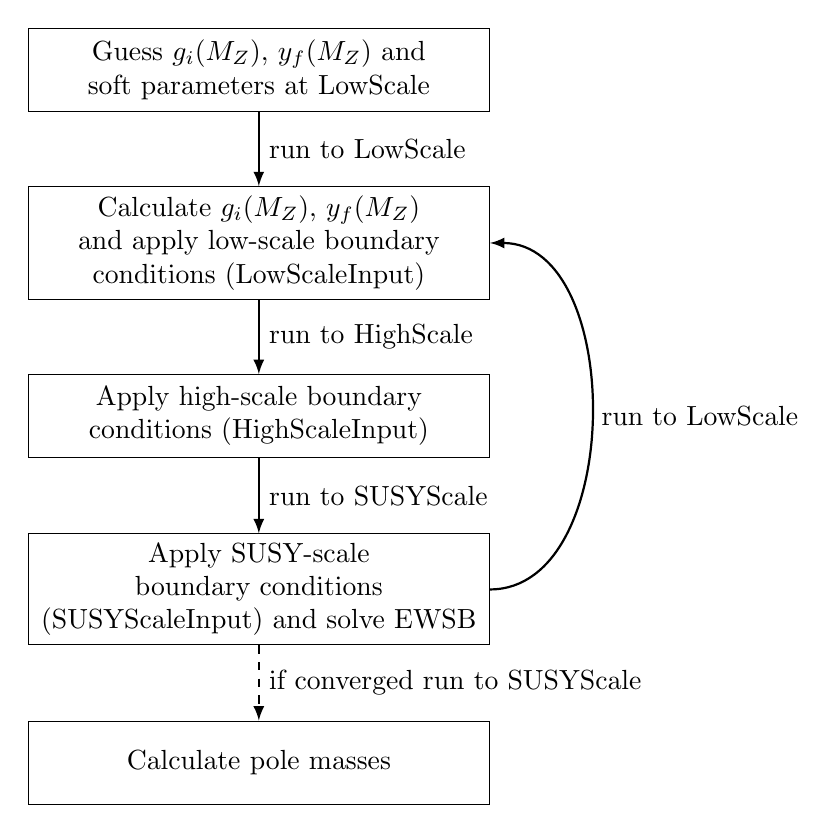
\begin{tikzpicture}[node distance = 2.2cm, auto]
    \tikzstyle{block} = [rectangle, draw, text width=16em, text centered, minimum height=3em]
    \tikzstyle{arrow} = [draw, -latex, thick]
    \node[block] (guess) {Guess $g_i(M_Z)$, $y_f(M_Z)$ and soft
      parameters at \code{LowScale}};
    \node[block,below of=guess] (MZ) {Calculate $g_i(M_Z)$, $y_f(M_Z)$ and apply
      low-scale boundary conditions (\code{LowScaleInput})};
    \path[arrow] (guess) -- node {run to \code{LowScale}} (MZ);
    \node[block,below of=MZ] (MX) {Apply high-scale boundary conditions
      (\code{HighScaleInput})};
    \path[arrow] (MZ) -- node {run to \code{HighScale}} (MX);
    \node[block,below of=MX] (MS) {Apply SUSY-scale boundary conditions
      (\code{SUSYScaleInput}) and solve EWSB};
    \path[arrow] (MX) -- node {run to \code{SUSYScale}} (MS);
    %\path[arrow] (MS.east) -| node {run to \code{LowScale}} (MZ.east);
    \path[-latex, thick] (MS.east) edge[bend right=90] node[right] {run to \code{LowScale}} (MZ.east);
    \node[block,below of=MS] (spec) {Calculate pole masses};
    \path[arrow,dashed] (MS) -- node[text width=16em] {if converged run to \code{SUSYScale}} (spec);
  \end{tikzpicture}
  \caption{Iterative two-scale algorithm to calculate the spectrum.}
  \label{fig:two-scale-algorithm}
\end{figure}

\subsection{Pole masses}
After the solver routine has finished and convergence has been
achieved, all $\overline{DR}$ parameters are consistent with the
one-loop EWSB conditions, low energy data and all user supplied
boundary conditions are known at any scale between \code{LowScale} and
\code{HighScale}.

The physical (pole) mass spectrum can now be calculated.  \fs uses the
full one-loop self-energies and tree-level mass matrices to calculate
the pole masses at the one-loop level, which means finding the values
$p$ that solve the equation
%
\begin{align}
  0 = \det\left[p^2\unity - m^2_{f,1L}(p^2)\right],
\end{align}
%
where the one-loop mass matrices $m_{f,1L}(p^2)$ are given in terms of
the tree-level mass matrices $m_f$ and the self-energies
$\Sigma_f(p^2)$ as
%
\begin{align}
  &\text{scalars } \phi: &
  m^2_{\phi,1L}(p^2) &= m^2_{\phi} - \Sigma_\phi(p^2), \\
  &\text{majorana fermions } \chi: &
  m_{\chi,1L}(p^2) &= m_{\chi} - \frac{1}{2}\Big[
    \Sigma_\chi^S(p^2) + \Sigma_\chi^{S,T}(p^2)
    + \Big( \Sigma_\chi^{L,T}(p^2) + \Sigma_\chi^R(p^2) \Big) m_{\chi} \notag \\
    &&&\phantom{= m_{\chi} - \frac{1}{2}\Big[}
    + m_{\chi} \Big( \Sigma_\chi^L(p^2) + \Sigma_\chi^{R,T}(p^2) \Big)
  \Big], \\
  &\text{dirac fermions } \psi: &
  m_{\psi,1L}(p^2) &= m_{\psi}
  - \Sigma_\psi^S(p^2)
  - \Sigma_\psi^R(p^2) m_{\psi}
  - m_{\psi} \Sigma_\psi^L(p^2) .
\end{align}
%
Since the one-loop mass matrices depend on $p$, an iterative procedure
must be used.  \fs provides three different methods with different
precision and execution speed to determine the mass eigenvalues:

\begin{itemize}
\item \code{LowDiagonalizationPrecision}: This option provides the
  lowest precision but is also the fastest one.  Here the one-loop
  mass matrix $m_{f,1L}^\text{low}$ is calculated exactly once as
%
  \begin{align}
    \forall i,j: (m_{f,1L}^\text{low})_{ij} = (m_{f,1L}(p^2 = m_{f_i}
    m_{f_j}))_{ij} ,
  \end{align}
%
  where $m_{f_i}$ is the $i$th mass eigenvalue of the tree-level mass
  matrix $m_f$.  Afterwards $m_{f,1L}^\text{low}$ is diagonalized and
  the eigenvalues are interpreted as pole masses $m_{f_i}^\pole$.

\item \code{MediumDiagonalizationPrecision} (default): This option
  provides calculation with medium precision with a medium execution
  time.  Here the one-loop mass matrix $m_{f,1L}^\text{medium}$ is
  calculated $n$ times as
%
  \begin{align}
    (m_{f,1L}^\text{medium})_{ij}^{(k)} = (m_{f,1L}(p^2 =
    m_{f_k}^2))_{ij} , \qquad k = 1,\ldots,n ,
  \end{align}
%
  where $m_{f_k}$ is the $k$th mass eigenvalue of the tree-level mass
  matrix $m_f$.  Afterwards, each mass matrix
  $(m_{f,1L}^\text{medium})^{(k)}$ is diagonalized and the $k$th
  eigenvalue is interpreted as pole mass $m_{f_k}^\pole$.

\item \code{HighDiagonalizationPrecision}: This option provides
  diagonalization with highest precision, but has also the highest
  execution time.  Here the one-loop mass matrix
  $m_{f,1L}^\text{high}$ is diagonalized $n$ times, as in the case of
  \code{MediumDiagonalizationPrecision}, resulting in $n$ pole masses
  $m_{f_k}^\pole$ ($k = 1,\ldots,n$).  Afterwards, the diagonalization
  is repeated, this time using the calculated pole masses
  $m_{f_k}^\pole$ for the momentum calculation $p^2 =
  (m_{f_k}^\pole)^2$.  The iteration stops until convergence is
  reached.
\end{itemize}

If higher accuracy is required additional routines with higher order
corrections can be added by setting \code{UseHiggs2LoopMSSM = True;}
in the model file. For example in the MSSM by default \fs adds
two-loop Higgs FORTRAN routines supplied by P.~Slavich from
\cite{Degrassi:2001yf,Brignole:2001jy,Dedes:2002dy,Brignole:2002bz,Dedes:2003km}
to add two-loop corrections of $\oatas$, $\oabas$, $\oatq$,
$\oabatau$, $\oabq$, $\oatauq$ and $\oatab$.

Something similar is done for the NMSSM, but in this case the NMSSM
$\oatas$, $\oabas$ pieces come from \cite{Degrassi:2009yq}, while for
$\oatq$, $\oabatau$, $\oabq$, $\oatauq$ and $\oatab$ the MSSM pieces
are used though it should be understood that these are not complete in
the NMSSM. For other models since the Higgs mass is a very important
measurement and the two loop corrections can be larger than the
current experimental error \cite{Degrassi:2009yq} we recommend that
the leading log two loop corrections are estimated, by generalising
those of the MSSM or NMSSM, as has been done, for example, in the
E$_6$SSM\cite{King:2005jy}.

\section{Flexible Spectra}
\label{Sec:Flexible}
\subsection{Meta code}
\subsection{Adapting C++ code}
\subsection{Combing with  modules of your own code}

\section{Run-time comparison with other spectrum generators}
\label{Sec:comparison}

One of \fs's design goals is a short run-time.  In this section we
demonstrate that this goal was achieved by comparing the run-time of
two different sets of CMSSM spectrum generators:
%
\begin{itemize}
\item \emph{Without flavour violation:} Disallowing flavour violation
  simplifies the calculation of the pole masses, because
  flavour-off-diagonal sfermion self-energy matrix elements don't need
  to be calculated.  Here we compare \fs's non-flavour violating CMSSM
  spectrum generator FlexibleSUSY-NoFV (version 1.0.0) against SPheno
  (version 3.2.4) and Softsusy (version 3.4.0).
%
\item \emph{With flavour violation:} Allowing for flavour violation in
  general increases the run-time of spectrum generators, because the
  full $6\times 6$ sfermion self-energy matrices have to be
  calculated.  Here we compare FlexibleSUSY-FV (version 1.0.0) and
  SPhenoMSSM (generated with SARAH 4.1.0 and linked against SPheno
  3.2.4).  Both spectrum generators are based on SARAH's MSSM model
  file, which allows for flavour violation.
\end{itemize}
%
FlexibleSUSY and Softsusy are compiled with g++ 4.8.0 and Intel ifort
13.1.3 20130607.  SPheno and SPhenoMSSM are compiled with Intel ifort
13.1.3 20130607.\footnote{Intel's ifort compiler decreases the
  run-time of SPheno and SPhenoMSSM by approximately a factor $1.5$,
  compared to gfortran.}

For the run-time comparison we're generating $2\cdot 10^{4}$ random
CMSSM parameter points with $m_0\in [50,1000]\unit{GeV}$, $m_{1/2}\in
[50,1000]\unit{GeV}$, $\tan\beta\in [1,100]$, $\sign\mu\in \{-1,+1\}$
and $A_0\in [-1000,1000]\unit{GeV}$.  For each point an SLHA input
file is created by appending the values of $m_0$, $m_{1/2}$,
$\tan\beta$, $\sign\mu$, $A_0$ in form of a \code{MINPAR} block to the
SLHA template file given in \ref{sec:speed-test-slha-template-file}.
The resulting SLHA input file is passed to each spectrum generator and
the (wall-clock) time is measured until the program has finished.  The
average run-times for three different CPU types can be found in
\tabref{tab:run-time-comparison}.  The first column shows the run-time
on a Intel Core2 Duo (P8600, $2.40\unit{GHz}$) where only one core was
enabled.  The second column shows the run-time on the same processor
where both cores were enabled.  In the third column a Intel Xeon
(L5640, $2.27\unit{GHz}$) was used, which has $6$ CPU cores.
%
\begin{table}[tbh]
  \centering
  \begin{tabular}{llll}
    \toprule
                            & Intel Core2 Duo    & Intel Core2 Duo   & Intel Xeon\\
                            & (P8600, 1 core)    & (P8600, 2 cores)  & (L5640, 6 cores)\\
    \midrule
    FlexibleSUSY-NoFV 1.0.0 & $0.086\unit{s}$    & $0.079\unit{s}$   & $0.060\unit{s}$\\
    SPheno 3.2.4            & $0.119\unit{s}$    & $0.114\unit{s}$   & $0.101\unit{s}$\\
    Softsusy 3.4.0          & $0.175\unit{s}$    & $0.171\unit{s}$   & $0.147\unit{s}$\\
    \midrule
    FlexibleSUSY-FV 1.0.0   & $0.150\unit{s}$    & $0.113\unit{s}$   & $0.074\unit{s}$\\
    SPhenoMSSM 4.1.0        & $0.415\unit{s}$    & $0.401\unit{s}$   & $0.370\unit{s}$\\
    \bottomrule
  \end{tabular}
  \caption{Average run-time of CMSSM spectrum generators for
    for random parameter points.  The first three rows show
    spectrum generators which disallow flavour violation.  Rows
    $4$--$5$ contain flavour violatig spectrum generators, based
    on SARAH's MSSM model file.}
  \label{tab:run-time-comparison}
\end{table}

Under both the non-flavour violating spectrum generators (first three
rows) as well as the flavour violating ones (4th and 5th row) we find
that \fs is significantly fastest.  Compared to SPheno,
FlexibleSUSY-NoFV is faster by a factor $1.4$--$1.7$, and compared to
Softsusy around a factor $2$--$2.5$.  Under the flavour violating
spectrum generators FlexibleSUSY-FV is faster than SPhenoMSSM by a
factor $2.8$--$5$.  Reason for the long run-time of SPhenoMSSM is the
long calculation duration of the two-loop $\beta$-functions.  Here \fs
benefits a lot from Eigen's well-optimizable matrix expressions.  We
also find that increasing the number of CPU cores reduces the run-time
of \fs.  The reason is that \fs calculates each pole mass in a
separate thread, and therefore benefits from multi-core CPUs.

\appendix
\section{Examples}
\subsection{NMSSM}
Detailed steps to create NMSSM model file.
\begin{enumerate}
\item Create new directory \code{mkdir myNMSSM}
\item Move into this new directory \code{cd myNMSSM}
\item copy the MSSM model file in \code{cp /path/to/SARAH/Models/MSSM/MSSM.m  myNMSSM.m}
\item Edit myNMSSM.m as follows
\begin{enumerate}
\item  Change Model name, author and date
\item Add singlet superfield to SuperFields
\begin{lstlisting}
SuperFields[[8]] = {s, 1, sR,    0, 1,  1, RpM};
\end{lstlisting}
\item Modify superpotential
\begin{lstlisting}
SuperPotential = Yu u.q.Hu - Yd d.q.Hd - Ye e.l.Hd + \[Lambda] s.Hu.Hd +  \[Kappa]/3 s.s.s ;
\end{lstlisting}
\item Add new VEV
\begin{lstlisting} 
  DEFINITION[EWSB][VEVs]= 
  { {SHd0, {vd, 1/Sqrt[2]}, {sigmad, \[ImaginaryI]/Sqrt[2]},{phid,1/Sqrt[2]}},
    {SHu0, {vu, 1/Sqrt[2]}, {sigmau, \[ImaginaryI]/Sqrt[2]},{phiu,1/Sqrt[2]}},
    {SsR,  {vs, 1/Sqrt[2]}, {sigmaS, \[ImaginaryI]/Sqrt[2]},{phiS,1/Sqrt[2]}}
};
\end{lstlisting}
\item  Add the singlino to the list of gauge eigenstate dirac fermions
\begin{lstlisting}
  DEFINITION[GaugeES][DiracSpinors]={
 .............
  FS -> {FsR,conj[FsR]}   
};
\end{lstlisting}
\item Edit mass eigenstates to give how the gauge eigenstates mix into mass eigenstates.  Here we add to the cp even higgs a real singlet, to the CP odd the imaginary part of the singlet and finally to the neutralinos we add the singlino.

\begin{lstlisting}
 DEFINITION[EWSB][MatterSector]= 
{   ................
    ................
     {{phid, phiu, phiS}, {hh, ZH}},      
     {{sigmad, sigmau, sigmaS}, {Ah, ZA}},
    ................
     {{fB, fW0, FHd0, FHu0, FsR}, {L0, ZN}},
     ...............
}; 

\end{lstlisting}
\end{enumerate}
\item Now we copy over particles.m \code{cp /path/to/SARAH/Models/MSSM/particles.m  ./}
\item Edit particles.m as follows
\begin{enumerate}  
\item First we add to particleDefinitions[GaugeES]:
\begin{lstlisting}
 ParticleDefinitions[GaugeES] = {
      {SsR, { Description -> "Singlet"}},        
      {FS,   { Description -> "Singlino" }},    
      ............
      };
\end{lstlisting}
Note that we are brief in information here becasue there is already some information contained in the default particles.m file in the model directory:
\begin{lstlisting} 
{{ Description -> "Singlet", 
                 PDG -> {0},
                 PDG.IX -> 0,
                 Width -> 0, 
                 Mass -> Automatic,
                 FeynArtsNr -> 98,
                 LaTeX -> "S",
                 OutputName -> "s"

    }},    
   
   
(* -------- Weyl Spinor  ------ *)   
    
  {{ Description -> "Weyl Spinor of Singlino", 
                 PDG -> 99,
                 Width -> 0, 
                 Mass -> Automatic,
                 FeynArtsNr -> 9,
                 LaTeX -> "\\tilde{S}",
                 OutputName -> "s"

    }},  

\end{lstlisting}
 \item Now we edit ParticleDefinitions[EWSB].  Again most states are defined in brief form by a name because they use the default information in the particles.m in the models directory.  But here we need to over write some of the default options for the cp even and cp odd higgs states: 
\begin{lstlisting}
 {hh   ,  {  Description -> "Higgs", 
                 PDG -> {25, 35,45},
                 PDG.IX ->{101000001,101000002,101000003}
 }}, 
       {Ah   ,  {    Description -> "Pseudo-Scalar Higgs",
                 PDG -> {0, 36, 46},
                 PDG.IX ->{0,102000001,102000002  } }}, 

\end{lstlisting}
\item To the WeylFermionAndIndermediate we add the Weyl singlino and the real scalar singlet field and imaginary scalar singlet field:  
 \begin{lstlisting}
  {sigmaS,      {Description -> "Scalar Singlet" }}  ,
  {phiS,      { Description -> "Pseudo Scalar Singlet"}},
  {FsR,   { Description -> "Weyl Spinor of Singlino"}},
 \end{lstlisting}
 
Although the WeylFermionAndIndermediate also contains, 
\begin{lstlisting}
{SHd,  { Description -> "Down-Higgs"}},
       {SHu,  { Description -> "Up-Higgs"}},
\end{lstlisting}
\noindent we do not add a singlet version becasue for the singlet there is no distinction between these and the individual SU(2) components, as there are for Hu and Hd.
\end{enumerate} 
\item Now we copy over parameters.m \code{cp /path/to/SARAH/Models/MSSM/parameters.m  ./}
\item Add the new parameters lambda, kappa, Alambda and Akappa to the list.
\begin{lstlisting}
{\[Kappa],   {Description -> "Singlet Self-Interaction"}},              
{T[\[Kappa]],  { Description -> "Softbreaking Singlet Self-Interaction" }}, 
{\[Lambda],   { Description -> "Singlet-Higgs-Interaction"   }},
{T[\[Lambda]],  {Description -> "Softbreaking Singlet-Higgs-Interaction"}}, 
{ms2,       { Description -> "Softbreaking Singlet Mass" }},
{vS,        { Description -> "Singlet-VEV"}}       
\end{lstlisting}
Once again this is simplified from the general case becasue there are default versions containedin parameters.m in the Models directory:
\begin{lstlisting}
{{  Description -> "Singlet Self-Interaction",
              LaTeX -> "\\kappa",
             Real ->False,
             Dependence -> None, 
             Value -> None, 
             LesHouches -> {NMSSMRUN,2},
             OutputName-> kap         }},                               
               
{{ Description -> "Softbreaking Singlet Self-Interaction",
               LaTeX -> "T_{\\kappa}",
              Real -> False,
             Dependence -> None, 
             Value -> None, 
             LesHouches ->{NMSSMRUN,4},
             OutputName-> Tk         }}, 

 {{ Description -> "Singlet-Higgs-Interaction",
             LaTeX -> "\\lambda",
             Real -> False,
	     Dependence -> None, 
             Value -> None, 
             LesHouches -> {NMSSMRUN,1},
             OutputName-> lam          }},                               
               
{{Description -> "Softbreaking Singlet-Higgs-Interaction",
                LaTeX -> "T_{\\lambda}",
              Real -> False,
             Dependence -> None, 
             Value -> None, 
             LesHouches ->{NMSSMRUN,3},
             OutputName-> Tlam         }},    
{{ Description -> "Softbreaking Singlet Mass", 
              LaTeX -> "m_S^2",
             DependenceNum ->  None, 
             LesHouches -> {NMSSMRUN,10},
             OutputName-> ms2 }},
              
{{ Description -> "Singlet-VEV", 
			 LaTeX -> "v_s",
             Value -> None, 
             LesHouches -> {NMSSMRUN,5},
             OutputName-> vS         }},
\end{lstlisting}
\item Navigate to Flexible SUSY directory  \code{cd /path/to/FlexibleSUSY/}
\item Create Z3NMSSM directory \code{./createmodel --models=Z3NMSSM:myNMSSM}
\item Configure with the new model \code{./configure --with-models=Z3NMSSM}
\item The default FlexibleSUSY model file for the MSSM will now be in the models/NMSSM2 directory.  Edit this for the NMSSM as follows:
  \begin{enumerate} 
    \item Add new input parameter $\lambda$ to EXTPAR and remove the sign of $\mu$ from MINPAR.
      \begin{lstlisting}    
        MINPAR = { {1, m0},
           {2, m12},
           {3, TanBeta},
           {5, Azero} };

  EXTPAR = { {61, LambdaInput} };
      \end{lstlisting}
     \item Also add this parameter to the DefaultParameterPoint.
      \begin{lstlisting}
       DefaultParameterPoint = {
    {m0, 200},
    {m12, 200},
    {TanBeta, 10},
    {Azero, -500}
    {LambdaInput, 0.1}
    };
  \end{lstlisting}
    \item Name the parameters you wish to be output by the EWSB conditions.  Note you should use the names given for them in parameters.m.    A common choice in the NMSSM is:
\begin{lstlisting}
EWSBOutputParameters = {vS, \[Kappa], ms2};
\end{lstlisting}
which will work for the semi-constrained NMSSM.
\item choose the Highscale and Highscale first guess, if the default is different from what you wish to use.  
\begin{lstlisting} 
 HighScale = g1 == g2;
 HighScaleFirstGuess = 2.0 10^16;
\end{lstlisting}
\item Add how the parameters found in parameters.m that are to be set at the highscale:
\begin{lstlisting} 
HighScaleInput={
   {T[Ye], Azero*Ye},
   {T[Yd], Azero*Yd},
   {T[Yu], Azero*Yu},
   {mHd2, m0^2},
   {mHu2, m0^2},
   {mq2, UNITMATRIX[3] m0^2},
   {ml2, UNITMATRIX[3] m0^2},
   {md2, UNITMATRIX[3] m0^2},
   {mu2, UNITMATRIX[3] m0^2},
   {me2, UNITMATRIX[3] m0^2},
   {MassB, m12},
   {MassWB,m12},
   {MassG,m12},
{\[Lambda], LambdaInput},
   {T[\[Kappa]], Azero \[Kappa]},
   {T[\[Lambda]], Azero LambdaInput}
};
\end{lstlisting}
\item set lowscale boundary condititions if you want something different from the default.  The defaults are:
\begin{lstlisting} 
 LowScale = SM[MZ];
 LowScaleFirstGuess = SM[MZ];
\end{lstlisting}
\item Change the LowscaleInput if necessary.  In this example we keep the same choice as in the MSSM
  \begin{lstlisting} 
 LowScaleInput={
   {vd, 2 MZDRbar / Sqrt[GUTNormalization[g1]^2 g1^2 + g2^2] Cos[ArcTan[TanBeta]]},
   {vu, 2 MZDRbar / Sqrt[GUTNormalization[g1]^2 g1^2 + g2^2] Sin[ArcTan[TanBeta]]}
};
  \end{lstlisting}

Finally we set the initial guesses for the paremeters.  In this example we overwtite the MSSM version replacing it with:
 \begin{lstlisting} 
InitialGuessAtLowScale = {
   {vd, SM[vev] Cos[ArcTan[TanBeta]]},
   {vu, SM[vev] Sin[ArcTan[TanBeta]]},
   {\[Lambda], LambdaInput},
   {\[Kappa], 0.1},
   {vS, 1000},
   {ms2, SM[MZ]^2}
};

InitialGuessAtHighScale = {};
 \end{lstlisting}

The code can now be created and also compiled (if you didn't select --disable-compile option when you ran the configure script) by typing \code{make -j2}.


 \end{enumerate}   

\end{enumerate}   
\subsection{\ESSM}
Detailed steps to create \ESSM model file.
\begin{enumerate}
\item Create new directory \code{mkdir myE6SSM}
\item Move into this new directory \code{cd myE6SSM}
\item copy the MSSM model file in \code{cp /path/to/SARAH/Models/MSSM/MSSM.m  myE6SSM.m}
\item Edit myE6SSM.m as follows
\begin{enumerate}
\item  Change Model name, author and date
\item Add new Vector superfield,
 \begin{lstlisting} 
   Gauge[[4]]={Bp,  U[1], Ncharge, g1p, False, RpM};
 \end{lstlisting}
\item Modify MSSM superfield definitions to include new charges.
\begin{lstlisting}
SuperFields[[1]] = {q, 3, {uL,  dL},     1/6, 2, 3, 1, RpM};  
SuperFields[[2]] = {l, 3, {vL,  eL},    -1/2, 2, 1, 2, RpM};
SuperFields[[3]] = {Hd,1, {Hd0, Hdm},   -1/2, 2, 1, -3, RpP};
SuperFields[[4]] = {Hu,1, {Hup, Hu0},    1/2, 2, 1, -2, RpP};
SuperFields[[5]] = {d, 3, conj[dR],    1/3, 1, -3, 2, RpM};
SuperFields[[6]] = {u, 3, conj[uR],   -2/3, 1, -3, 1, RpM};
SuperFields[[7]] = {e, 3, conj[eR],      1, 1,  1, 1, RpM};
\end{lstlisting}
Note that in the \ESSM model the charges are fixed to be those of the $U(1)_N$ as shown in e.g. \cite{King:2005jy}.  However here one can leave the charges unassigned vby using parameters in place of the fixed charges.  Here we fix the charges to simplify the C++ code.

\item Add Singlet Higgs superfield to SuperField
\begin{lstlisting}
SuperFields[[8]] = {s, 1, sR,     0, 1,  1, 5, RpP};
\end{lstlisting}
\item Add inert Higgs-like superfields 
\begin{lstlisting}
SuperFields[[9]] = {H1I, 2, {H1I0, H1Im},  -1/2, 2, 1, -3, RpP};
SuperFields[[10]] = {H2I, 2, {H2Ip, H2I0},   1/2, 2, 1, -2, RpP};
SuperFields[[11]] = {sI, 2, sIR,    0, 1,  1, 5, RpM};
\end{lstlisting}
\item Add exotics to SuperFields
\begin{lstlisting}
SuperFields[[12]] = {Dx, 3, DxL,  -1/3, 1, 3, -2, RpP};
SuperFields[[13]] = {Dxbar, 3, conj[DxbarR],  1/3, 1, -3, -3, RpP};
\end{lstlisting}
\item Add additional survival $SU(2)$ multiplets to SuperFields
\begin{lstlisting}
SuperFields[[14]] = {Hp, 1, {Hpd0, Hpdm},  1/2, 2,  1, 2, RpP};
SuperFields[[15]] = {Hpbar, 1, {Hpup, Hpu0}, -1/2, 2,  1, -2, RpP};
\end{lstlisting}
\item Modify superpotential
\begin{lstlisting}
SuperPotential = Yu u.q.Hu - Yd d.q.Hd - Ye e.l.Hd + \[Lambda] s.Hu.Hd +  \[Lambda]12 s.H2I.H1I + \[Kappa] s.Dx.Dxbar + \[Mu]Pr Hp.Hpbar;
\end{lstlisting}
\item Define new gauge eigenstate Dirac spinors
\begin{lstlisting}
  DEFINITION[GaugeES][DiracSpinors]={
    .............
    .............
    FS -> {FsR,conj[FsR]},
    FBp -> {fBp,conj[fBp]},
    HI0 -> {FH1I0, conj[FH2I0]},
    HIC -> {FH1Im, conj[FH2Ip]},
    FSI -> {FsIR, conj[FsIR]},
    FDx1 -> {FDxL, 0},
    FDx2 -> {0, FDxbarR}, 
    Hp0 -> {FHpd0, conj[FHpu0]},
    HpC -> {FHpdm, conj[FHpup]}
  };
\end{lstlisting}
\item Add new VEV
\begin{lstlisting} 
  DEFINITION[EWSB][VEVs]= 
  { {SHd0, {vd, 1/Sqrt[2]}, {sigmad, \[ImaginaryI]/Sqrt[2]},{phid,1/Sqrt[2]}},
    {SHu0, {vu, 1/Sqrt[2]}, {sigmau, \[ImaginaryI]/Sqrt[2]},{phiu,1/Sqrt[2]}},
    {SsR,  {vs, 1/Sqrt[2]}, {sigmaS, \[ImaginaryI]/Sqrt[2]},{phiS,1/Sqrt[2]}}
};
\end{lstlisting}
\item Add new gauge boson  mass eigenstate
\begin{lstlisting} 
  DEFINITION[EWSB][GaugeSector] =
  { 
    {{VB,VWB[3],VBp},{VP,VZ,VZp},ZZ},
    {{VWB[1],VWB[2]},{VWm,conj[VWm]},ZW},
    {{fWB[1],fWB[2],fWB[3]},{fWm,fWp,fW0},ZfW}
  }; 
\end{lstlisting}
\item Edit mixings for Higgs and neutralino states and add additional states that mix.
\begin{lstlisting}
DEFINITION[EWSB][MatterSector]= 
{ ...............
  ...............
{{phid, phiu, phiS}, {hh, ZH}},
{{sigmad, sigmau, sigmaS}, {Ah, ZA}},
  ...............
{{fB, fW0, FHd0, FHu0, FsR, fBp}, {L0, ZN}},
 ................ 
 {{SH1I0,conj[SH2I0]},{SHI0,UHI0}},
 {{SH1Im,conj[SH2Ip]},{SHIp,UHIp}},
 {{SHpd0,conj[SHpu0]},{SHp0,UHp0}},
 {{SHpdm,conj[SHpup]},{SHpp,UHpp}},
 {{FHpd0,FHpu0},{L0p,ZNp}},
 {{FH1I0,FH2I0},{L0I,ZNI}}
\end{lstlisting}
\end{enumerate}  
 
\end{enumerate}   

\section{Numeric tests}

For checking the correctness of \fs's generated spectrum generators
extensive unit tests against Softsusy's MSSM, and NMSSM
implementations (both $Z_3$-invariant and $Z_3$-violating variants)
were done: We checked mass matrices, EWSB equations, one- and two-loop
$\beta$-functions, one- and two-loop self-energies and one- and
two-loop tadpoles and found all to agree within double machine
precision.  We also compared the overall pole mass spectrum after the
full fixed-point iteration has finished, and found the spectra to
agree at the sub-permille level.  Analytic tests of the $R$-symmetric
low-energy model, MRSSM, were done by Philip Diessner and several bugs
in \fs and SARAH were identified and fixed.

TODO: Adding tests against the CE$_6$SSM?

We also compared the run-time of \fs against SPheno, Softsusy and the
SARAH generated MSSM spectrum generator SPhenoMSSM.  The test results
can be found in \secref{Sec:comparison}.

\section{Speed test SLHA input file}
\label{sec:speed-test-slha-template-file}
%
\begin{lstlisting}
Block MODSEL                 # Select model
    6    0                   # flavour violation
    1    1                   # mSUGRA
Block SMINPUTS               # Standard Model inputs
    1   1.279180000e+02      # alpha^(-1) SM MSbar(MZ)
    2   1.166390000e-05      # G_Fermi
    3   1.189000000e-01      # alpha_s(MZ) SM MSbar
    4   9.118760000e+01      # MZ(pole)
    5   4.200000000e+00      # mb(mb) SM MSbar
    6   1.709000000e+02      # mtop(pole)
    7   1.777000000e+00      # mtau(pole)
Block SOFTSUSY               # SOFTSUSY specific inputs
    1   1.000000000e-04      # tolerance
    2   2                    # up-quark mixing (=1) or down (=2)
    3   0                    # printout
    5   1                    # 2-loop running
    7   2                    # EWSB and Higgs mass loop order
Block FlexibleSUSY
    0   1.000000000e-04      # precision goal
    1   0                    # max. iterations (0 = automatic)
    2   0                    # algorithm (0 = two_scale, 1 = lattice)
    3   0                    # calculate SM pole masses
    4   2                    # pole mass loop order
    5   2                    # EWSB loop order
    6   2                    # beta-functions loop order
Block SPhenoInput            # SPheno specific input
    1  -1                    # error level
    2   1                    # SPA conventions
    11  0                    # calculate branching ratios
    13  0                    # include 3-Body decays
    12  1.000E-04            # write only branching ratios larger than this value
    31  -1                   # fixed GUT scale (-1: dynamical GUT scale)
    32  0                    # Strict unification
    34  1.000E-04            # Precision of mass calculation
    35  40                   # Maximal number of iterations
    37  1                    # Set Yukawa scheme
    38  2                    # 1- or 2-Loop RGEs
    50  1                    # Majorana phases: use only positive masses
    51  0                    # Write Output in CKM basis
    52  0                    # Write spectrum in case of tachyonic states
    55  1                    # Calculate one loop masses
    57  0                    # Calculate low energy constraints
    60  0                    # Include possible, kinetic mixing
    65  1                    # Solution tadpole equation
    75  0                    # Write WHIZARD files
    76  0                    # Write HiggsBounds file
    86  0.                   # Maximal width to be counted as invisible in Higgs decays
    510 0.                   # Write tree level values for tadpole solutions
    515 0                    # Write parameter values at GUT scale
    520 0.                   # Write effective Higgs couplings (HiggsBounds blocks)
    525 0.                   # Write loop contributions to diphoton decay of Higgs
Block MINPAR
    1   [50..1000]           # m0(MX)
    2   [50..1000]           # m12(MX)
    3   [1..100]             # tan(beta)(MZ) DRbar
    4   {-1,+1}              # sign(mu)
    5   [-1000..1000]        # A0(MX)
\end{lstlisting}

\clearpage
\section*{References}

\begin{thebibliography}{100}
%% %\cite{Nilles:1983ge}
%% \bibitem{Nilles:1983ge} 
%%   H.~P.~Nilles,
%%   %``Supersymmetry, Supergravity and Particle Physics,''
%%   Phys.\ Rept.\  {\bf 110}, 1 (1984).
%%   %%CITATION = PRPLC,110,1;%%
%%   %4282 citations counted in INSPIRE as of 24 Apr 2014
%% %\cite{Lahanas:1986uc}
%% \bibitem{Lahanas:1986uc} 
%%   A.~B.~Lahanas and D.~V.~Nanopoulos,
%%   %``The Road to No Scale Supergravity,''
%%   Phys.\ Rept.\  {\bf 145}, 1 (1987).
%%   %%CITATION = PRPLC,145,1;%%
%%   %694 citations counted in INSPIRE as of 24 Apr 2014
%% %\cite{Ellis:1990wk}
%\cite{Coleman:1967ad}
\bibitem{Coleman:1967ad} 
  S.~R.~Coleman and J.~Mandula,
  %``All Possible Symmetries of the S Matrix,''
  Phys.\ Rev.\  {\bf 159}, 1251 (1967).
  %%CITATION = PHRVA,159,1251;%%
  %722 citations counted in INSPIRE as of 24 Apr 2014
%\cite{Haag:1974qh}
\bibitem{Haag:1974qh} 
  R.~Haag, J.~T.~Lopuszanski and M.~Sohnius,
  %``All Possible Generators of Supersymmetries of the s Matrix,''
  Nucl.\ Phys.\ B {\bf 88}, 257 (1975).
  %%CITATION = NUPHA,B88,257;%%
  %828 citations counted in INSPIRE as of 24 Apr 2014
%\cite{Weinberg:1975gm}
\bibitem{Weinberg:1975gm} 
  S.~Weinberg,
  %``Implications of Dynamical Symmetry Breaking,''
  Phys.\ Rev.\ D {\bf 13}, 974 (1976).
  %%CITATION = PHRVA,D13,974;%%
  %1251 citations counted in INSPIRE as of 24 Apr 2014
%\cite{Weinberg:1979bn}
\bibitem{Weinberg:1979bn}
  S.~Weinberg,
  %``Implications of Dynamical Symmetry Breaking: An Addendum,''
  Phys.\ Rev.\ D {\bf 19} (1979) 1277.
  %%CITATION = PHRVA,D19,1277;%%
  %1586 citations counted in INSPIRE as of 24 Apr 2014
%\cite{Gildener:1976ai}
\bibitem{Gildener:1976ai} 
  E.~Gildener,
  %``Gauge Symmetry Hierarchies,''
  Phys.\ Rev.\ D {\bf 14}, 1667 (1976).
  %%CITATION = PHRVA,D14,1667;%%
  %480 citations counted in INSPIRE as of 24 Apr 2014
%\cite{Susskind:1978ms}
\bibitem{Susskind:1978ms}
  L.~Susskind,
  %``Dynamics of Spontaneous Symmetry Breaking in the Weinberg-Salam Theory,''
  Phys.\ Rev.\ D {\bf 20} (1979) 2619.
  %%CITATION = PHRVA,D20,2619;%%
  %2011 citations counted in INSPIRE as of 24 Apr 2014
%\cite{'tHooft:1980xb}
\bibitem{'tHooft:1980xb} 
  G.~'t Hooft, C.~Itzykson, A.~Jaffe, H.~Lehmann, P.~K.~Mitter, I.~M.~Singer and R.~Stora,
  %``Recent Developments in Gauge Theories. Proceedings, Nato Advanced Study Institute, Cargese, France, August 26 - September 8, 1979,''
  NATO Adv.\ Study Inst.\ Ser.\ B Phys.\  {\bf 59}, pp.1 (1980).
  %%CITATION = NASBD,59,pp.1;%%
  %10 citations counted in INSPIRE as of 24 Apr 2014

\bibitem{Langacker:1990jh} 
  P.~Langacker,
  %``Precision tests of the standard model,''
  In *Boston 1990, Proceedings, Particles, strings and cosmology* 237-269 and Pennsylvania Univ. Philadelphia - UPR-0435T (90,rec.Oct.) 33 p. (015721) (see HIGH ENERGY PHYSICS INDEX 29 (1991) No. 9950)
  %4 citations counted in INSPIRE as of 24 Apr 2014

\bibitem{Ellis:1990wk} 
  J.~R.~Ellis, S.~Kelley and D.~V.~Nanopoulos,
  %``Probing the desert using gauge coupling unification,''
  Phys.\ Lett.\ B {\bf 260}, 131 (1991).
  %%CITATION = PHLTA,B260,131;%%
  %862 citations counted in INSPIRE as of 24 Apr 2014
%\cite{Amaldi:1991cn}
\bibitem{Amaldi:1991cn} 
  U.~Amaldi, W.~de Boer and H.~Furstenau,
  %``Comparison of grand unified theories with electroweak and strong coupling constants measured at LEP,''
  Phys.\ Lett.\ B {\bf 260}, 447 (1991).
  %%CITATION = PHLTA,B260,447;%%
  %1525 citations counted in INSPIRE as of 24 Apr 2014
%\cite{Langacker:1991an}
\bibitem{Langacker:1991an} 
  P.~Langacker and M.~-x.~Luo,
  %``Implications of precision electroweak experiments for $M_t$, $\rho_{0}$, $\sin^2\theta_W$ and grand unification,''
  Phys.\ Rev.\ D {\bf 44}, 817 (1991).
  %%CITATION = PHRVA,D44,817;%%
  %1219 citations counted in INSPIRE as of 24 Apr 2014
%\cite{Giunti:1991ta}
\bibitem{Giunti:1991ta} 
  C.~Giunti, C.~W.~Kim and U.~W.~Lee,
  %``Running coupling constants and grand unification models,''
  Mod.\ Phys.\ Lett.\ A {\bf 6}, 1745 (1991).
  %%CITATION = MPLAE,A6,1745;%%
  %273 citations counted in INSPIRE as of 24 Apr 2014
%\cite{Langacker:1990jh}


%\cite{Goldberg:1983nd}
\bibitem{Goldberg:1983nd} 
  H.~Goldberg,
  %``Constraint on the Photino Mass from Cosmology,''
  Phys.\ Rev.\ Lett.\  {\bf 50}, 1419 (1983)
  [Erratum-ibid.\  {\bf 103}, 099905 (2009)].
  %%CITATION = PRLTA,50,1419;%%
  %972 citations counted in INSPIRE as of 24 Apr 2014
%\cite{Ellis:1983ew}
\bibitem{Ellis:1983ew} 
  J.~R.~Ellis, J.~S.~Hagelin, D.~V.~Nanopoulos, K.~A.~Olive and M.~Srednicki,
  %``Supersymmetric Relics from the Big Bang,''
  Nucl.\ Phys.\ B {\bf 238}, 453 (1984).
  %%CITATION = NUPHA,B238,453;%%
  %1282 citations counted in INSPIRE as of 24 Apr 2014

%\cite{Girardello:1981wz}
\bibitem{Girardello:1981wz}
  L.~Girardello and M.~T.~Grisaru,
  %``Soft Breaking of Supersymmetry,''
  Nucl.\ Phys.\ B {\bf 194} (1982) 65.
  %%CITATION = NUPHA,B194,65;%%
  %717 citations counted in INSPIRE as of 21 Feb 2014

%\cite{Allanach:2001kg}
\bibitem{Allanach:2001kg} 
  B.~C.~Allanach,
  %``SOFTSUSY: a program for calculating supersymmetric spectra,''
  Comput.\ Phys.\ Commun.\  {\bf 143}, 305 (2002)
  [hep-ph/0104145].
  %%CITATION = HEP-PH/0104145;%%
  %716 citations counted in INSPIRE as of 20 Sep 2013
%\cite{Porod:2003um}
\bibitem{Porod:2003um} 
  W.~Porod,
  %``SPheno, a program for calculating supersymmetric spectra, SUSY particle decays and SUSY particle production at e+ e- colliders,''
  Comput.\ Phys.\ Commun.\  {\bf 153}, 275 (2003)
  [hep-ph/0301101].
  %%CITATION = HEP-PH/0301101;%%
  %413 citations counted in INSPIRE as of 03 Nov 2013

%\cite{Djouadi:2002ze}
\bibitem{Djouadi:2002ze} 
  A.~Djouadi, J.~-L.~Kneur and G.~Moultaka,
  %``SuSpect: A Fortran code for the supersymmetric and Higgs particle spectrum in the MSSM,''
  Comput.\ Phys.\ Commun.\  {\bf 176}, 426 (2007)
  [hep-ph/0211331].
  %%CITATION = HEP-PH/0211331;%%
  %654 citations counted in INSPIRE as of 03 Nov 2013

%\cite{Baer:1993ae}
\bibitem{Baer:1993ae} 
  H.~Baer, F.~E.~Paige, S.~D.~Protopopescu and X.~Tata,
  %``Simulating Supersymmetry with ISAJET 7.0 / ISASUSY 1.0,''
  hep-ph/9305342.
  %%CITATION = HEP-PH/9305342;%%
  %82 citations counted in INSPIRE as of 03 Nov 2013
%\cite{Ellwanger:2006rn}
\bibitem{Ellwanger:2006rn} 
  U.~Ellwanger and C.~Hugonie,
  %``NMSPEC: A Fortran code for the sparticle and Higgs masses in the NMSSM with GUT scale boundary conditions,''
  Comput.\ Phys.\ Commun.\  {\bf 177}, 399 (2007)
  [hep-ph/0612134].
  %%CITATION = HEP-PH/0612134;%%
  %81 citations counted in INSPIRE as of 03 Nov 2013
%\cite{Allanach:2013kza}
\bibitem{Allanach:2013kza} 
  B.~C.~Allanach, P.~Athron, L.~C.~Tunstall, A.~Voigt and A.~G.~Williams,
  %``Next-to-Minimal SOFTSUSY,''
  arXiv:1311.7659 [hep-ph].
  %%CITATION = ARXIV:1311.7659;%%
  %1 citations counted in INSPIRE as of 24 Apr 2014
\bibitem{NMSSM} P. Fayet, Nucl. Phys. B \textbf{90} (1975) 104; Phys. Lett.
B \textbf{64} (1976) 159; Phys. Lett. B \textbf{69} (1977) 489 and Phys. Lett. B
\textbf{84} (1979) 416; H.P. Nilles, M. Srednicki and D. Wyler, Phys. Lett. B
\textbf{120} (1983) 346; J.M. Frere, D.R. Jones and S. Raby, Nucl. Phys. B
\textbf{222} (1983) 11; J.P. Derendinger and C.A. Savoy, Nucl. Phys. B
\textbf{237} (1984) 307;  A.I. Veselov, M.I. Vysotsky and K.A. Ter-Martirosian,
Sov. Phys. JETP \textbf{63} (1986) 489; J.R. Ellis, J.F. Gunion, H.E. Haber, L.
Roszkowski and F. Zwirner, Phys. Rev. D \textbf{39}  (1989) 844; M. Drees, Int.
J. Mod. Phys. A \textbf{4}  (1989) 3635; U. Ellwanger, M. Rausch de
Traubenberg and C.A. Savoy, Phys. 
Lett. B \textbf{315} (1993) 331, Z. Phys. C {\bf 67} (1995) 665 and Nucl. Phys.
B \textbf{492} (1997) 307; U.~Ellwanger, Phys.\ Lett.\  B {\bf 303} (1993) 271; P.
Pandita, Z. Phys. C \textbf{59} (1993) 575; T. Elliott, S.F. King and P.L.
White, Phys. Rev. D {\bf 49} (1994) 2435; S.F. King and P.L. White, Phys. Rev. D
\textbf{52} (1995) 4183;  F.~Franke and H.~Fraas, Int.\ J.\ Mod.\ Phys.\  A {\bf
12} (1997) 479.   D.~J.~Miller, R.~Nevzorov and P.~M.~Zerwas,  Nucl.\ Phys.\ B {\bf 681}, 3 (2004) [hep-ph/0304049].
%\cite{Kim:1983dt}
\bibitem{Kim:1983dt} 
  J.~E.~Kim and H.~P.~Nilles,
  %``The mu Problem and the Strong CP Problem,''
  Phys.\ Lett.\ B {\bf 138}, 150 (1984).
  %%CITATION = PHLTA,B138,150;%%
  %604 citations counted in INSPIRE as of 24 Apr 2014
%\cite{King:2014nza}
\bibitem{King:2014nza} 
  S.~F.~King, A.~Merle, S.~Morisi, Y.~Shimizu and M.~Tanimoto,
  %``Neutrino Mass and Mixing: from Theory to Experiment,''
  arXiv:1402.4271 [hep-ph].
  %%CITATION = ARXIV:1402.4271;%%
  %9 citations counted in INSPIRE as of 24 Apr 2014
%\cite{King:2008qb}
\bibitem{King:2008qb} 
  S.~F.~King, R.~Luo, D.~J.~Miller and R.~Nevzorov,
  %``Leptogenesis in the Exceptional Supersymmetric Standard Model: Flavour dependent lepton asymmetries,''
  JHEP {\bf 0812}, 042 (2008)
  [arXiv:0806.0330 [hep-ph]].
  %%CITATION = ARXIV:0806.0330;%%
  %26 citations counted in INSPIRE as of 24 Apr 2014
%\cite{Aad:2013wta}
\bibitem{Aad:2013wta} 
  G.~Aad {\it et al.}  [ATLAS Collaboration],
  %``Search for new phenomena in final states with large jet multiplicities and missing transverse momentum at sqrt(s)=8 TeV proton-proton collisions using the ATLAS experiment,''
  JHEP {\bf 1310}, 130 (2013)
  [arXiv:1308.1841 [hep-ex]].
  %%CITATION = ARXIV:1308.1841;%%
  %36 citations counted in INSPIRE as of 24 Apr 2014
\bibitem{Chatrchyan:2014lfa}
  S.~Chatrchyan {\it et al.}  [CMS Collaboration],
  %``Search for new physics in the multijet and missing transverse momentum final state in proton-proton collisions at $\sqrt{s}$ = 8 TeV,''
  arXiv:1402.4770 [hep-ex].
  %%CITATION = ARXIV:1402.4770;%%
  %10 citations counted in INSPIRE as of 24 Apr 2014
%\cite{ATLAS:2012ae}
\bibitem{ATLAS:2012ae} 
  G.~Aad {\it et al.}  [ATLAS Collaboration],
  %``Combined search for the Standard Model Higgs boson using up to 4.9 fb$^{-1}$ of $pp$ collision data at $\sqrt{s}=7$ TeV with the ATLAS detector at the LHC,''
  Phys.\ Lett.\ B {\bf 710}, 49 (2012)
  [arXiv:1202.1408 [hep-ex]].
  %%CITATION = ARXIV:1202.1408;%%
  %474 citations counted in INSPIRE as of 24 Apr 2014
%\cite{Chatrchyan:2012tx}
\bibitem{Chatrchyan:2012tx} 
  S.~Chatrchyan {\it et al.}  [CMS Collaboration],
  %``Combined results of searches for the standard model Higgs boson in $pp$ collisions at $\sqrt{s}=7$ TeV,''
  Phys.\ Lett.\ B {\bf 710}, 26 (2012)
  [arXiv:1202.1488 [hep-ex]].
  %%CITATION = ARXIV:1202.1488;%%
  %592 citations counted in INSPIRE as of 24 Apr 2014
%\cite{Chatrchyan:2014lfa}
 %\cite{Staub:2010ty}
\bibitem{Staub:2010ty} 
  F.~Staub, W.~Porod and B.~Herrmann,
  %``The Electroweak sector of the NMSSM at the one-loop level,''
  JHEP {\bf 1010}, 040 (2010)
  [arXiv:1007.4049 [hep-ph]].
  %%CITATION = ARXIV:1007.4049;%%
  %28 citations counted in INSPIRE as of 12 Oct 2013

%\cite{Staub:2009bi}
\bibitem{Staub:2009bi} 
  F.~Staub,
  %``From Superpotential to Model Files for FeynArts and CalcHep/CompHep,''
  Comput.\ Phys.\ Commun.\  {\bf 181}, 1077 (2010)
  [arXiv:0909.2863 [hep-ph]].
  %%CITATION = ARXIV:0909.2863;%%
  %64 citations counted in INSPIRE as of 12 Oct 2013

%\cite{Staub:2010jh}
\bibitem{Staub:2010jh} 
  F.~Staub,
  %``Automatic Calculation of supersymmetric Renormalization Group Equations and Self Energies,''
  Comput.\ Phys.\ Commun.\  {\bf 182}, 808 (2011)
  [arXiv:1002.0840 [hep-ph]].
  %%CITATION = ARXIV:1002.0840;%%
  %60 citations counted in INSPIRE as of 12 Oct 2013

%\cite{Staub:2012pb}
\bibitem{Staub:2012pb} 
  F.~Staub,
  %``SARAH 3.2: Dirac Gauginos, UFO output, and more,''
  Computer Physics Communications {\bf 184}, pp. 1792 (2013)
  [Comput.\ Phys.\ Commun.\  {\bf 184}, 1792 (2013)]
  [arXiv:1207.0906 [hep-ph]].
  %%CITATION = ARXIV:1207.0906;%%
  %19 citations counted in INSPIRE as of 12 Oct 2013

%\cite{Staub:2013tta}
\bibitem{Staub:2013tta} 
  F.~Staub,
  %``SARAH 4: A tool for (not only SUSY) model builders,''
  arXiv:1309.7223 [hep-ph].
  %%CITATION = ARXIV:1309.7223;%%
  %2 citations counted in INSPIRE as of 12 Oct 2013

%\cite{Degrassi:2009yq}
\bibitem{Degrassi:2009yq} 
  G.~Degrassi and P.~Slavich,
  %``On the radiative corrections to the neutral Higgs boson masses in the NMSSM,''
  Nucl.\ Phys.\ B {\bf 825}, 119 (2010)
  [arXiv:0907.4682 [hep-ph]].
  %%CITATION = ARXIV:0907.4682;%%
  %35 citations counted in INSPIRE as of 21 Sep 2013

%\cite{Skands:2003cj}
\bibitem{Skands:2003cj}
  P.~Z.~Skands, B.~C.~Allanach, H.~Baer, C.~Balazs, G.~Belanger, F.~Boudjema, A.~Djouadi and R.~Godbole {\it et al.},
  %``SUSY Les Houches accord: Interfacing SUSY spectrum calculators, decay packages, and event generators,''
  JHEP {\bf 0407} (2004) 036
  [hep-ph/0311123].
  %%CITATION = HEP-PH/0311123;%%
  %394 citations counted in INSPIRE as of 22 Feb 2014

%\cite{Allanach:2008qq}
\bibitem{Allanach:2008qq} 
  B.~C.~Allanach, C.~Balazs, G.~Belanger, M.~Bernhardt, F.~Boudjema, D.~Choudhury, K.~Desch and U.~Ellwanger {\it et al.},
  %``SUSY Les Houches Accord 2,''
  Comput.\ Phys.\ Commun.\  {\bf 180}, 8 (2009)
  [arXiv:0801.0045 [hep-ph]].
  %%CITATION = ARXIV:0801.0045;%%
  %177 citations counted in INSPIRE as of 21 Sep 2013

%\cite{Ellwanger:2009dp}
\bibitem{Ellwanger:2009dp} 
  U.~Ellwanger, C.~Hugonie and A.~M.~Teixeira,
  %``The Next-to-Minimal Supersymmetric Standard Model,''
  Phys.\ Rept.\  {\bf 496}, 1 (2010)
  [arXiv:0910.1785 [hep-ph]].
  %%CITATION = ARXIV:0910.1785;%%
  %327 citations counted in INSPIRE as of 21 Sep 2013

%\cite{Jones:1974pg}
\bibitem{Jones:1974pg}
  D.~R.~T.~Jones,
  %``Asymptotic Behavior of Supersymmetric Yang-Mills Theories in the Two Loop Approximation,''
  Nucl.\ Phys.\ B {\bf 87} (1975) 127.
  %%CITATION = NUPHA,B87,127;%%
  %123 citations counted in INSPIRE as of 21 Feb 2014

%\cite{Jones:1983vk}
\bibitem{Jones:1983vk}
  D.~R.~T.~Jones and L.~Mezincescu,
  %``The Beta Function in Supersymmetric {Yang-Mills} Theory,''
  Phys.\ Lett.\ B {\bf 136} (1984) 242.
  %%CITATION = PHLTA,B136,242;%%
  %109 citations counted in INSPIRE as of 21 Feb 2014

%\cite{West:1984dg}
\bibitem{West:1984dg}
  P.~C.~West,
  %``The Yukawa beta Function in N=1 Rigid Supersymmetric Theories,''
  Phys.\ Lett.\ B {\bf 137} (1984) 371.
  %%CITATION = PHLTA,B137,371;%%
  %134 citations counted in INSPIRE as of 21 Feb 2014

%\cite{Martin:1993yx}
\bibitem{Martin:1993yx}
  S.~P.~Martin and M.~T.~Vaughn,
  %``Regularization dependence of running couplings in softly broken supersymmetry,''
  Phys.\ Lett.\ B {\bf 318} (1993) 331
  [hep-ph/9308222].
  %%CITATION = HEP-PH/9308222;%%
  %220 citations counted in INSPIRE as of 21 Feb 2014

%\cite{Yamada:1993ga}
\bibitem{Yamada:1993ga}
  Y.~Yamada,
  %``Two loop renormalization of gaugino masses in general supersymmetric gauge models,''
  Phys.\ Rev.\ Lett.\  {\bf 72} (1994) 25
  [hep-ph/9308304].
  %%CITATION = HEP-PH/9308304;%%
  %48 citations counted in INSPIRE as of 21 Feb 2014

%\cite{MV94}
\bibitem{MV94} 
  S.~P.~Martin and M.~T.~Vaughn,
  %``Two loop renormalization group equations for soft supersymmetry breaking couplings,''
  Phys.\ Rev.\ D {\bf 50}, 2282 (1994)
  [Erratum-ibid.\ D {\bf 78}, 039903 (2008)]
  [hep-ph/9311340].
  %%CITATION = HEP-PH/9311340;%%
  %568 citations counted in INSPIRE as of 24 Sep 2013

%\cite{Fonseca:2011vn}
\bibitem{Fonseca:2011vn}
  R.~M.~Fonseca, M.~Malinsky, W.~Porod and F.~Staub,
  %``Running soft parameters in SUSY models with multiple U(1) gauge factors,''
  Nucl.\ Phys.\ B {\bf 854} (2012) 28
  [arXiv:1107.2670 [hep-ph]].
  %%CITATION = ARXIV:1107.2670;%%
  %29 citations counted in INSPIRE as of 21 Feb 2014

%\cite{Yam94}
\bibitem{Yam94} 
  Y.~Yamada,
  %``Two loop renormalization group equations for soft SUSY breaking scalar interactions: Supergraph method,''
  Phys.\ Rev.\ D {\bf 50}, 3537 (1994)
  [hep-ph/9401241].
  %%CITATION = HEP-PH/9401241;%%
  %225 citations counted in INSPIRE as of 24 Sep 2013

%\cite{Sperling:2013eva}
\bibitem{Sperling:2013eva}
  M.~Sperling, D.~Stöckinger and A.~Voigt,
  %``Renormalization of vacuum expectation values in spontaneously broken gauge theories,''
  JHEP {\bf 1307} (2013) 132
  [arXiv:1305.1548 [hep-ph]].
  %%CITATION = ARXIV:1305.1548;%%
  %10 citations counted in INSPIRE as of 21 Feb 2014

%\cite{Sperling:2013xqa}
\bibitem{Sperling:2013xqa}
  M.~Sperling, D.~Stöckinger and A.~Voigt,
  %``Renormalization of vacuum expectation values in spontaneously broken gauge theories: Two-loop results,''
  JHEP {\bf 1401} (2014) 068
  [arXiv:1310.7629 [hep-ph]].
  %%CITATION = ARXIV:1310.7629;%%
  %4 citations counted in INSPIRE as of 21 Feb 2014

%\cite{Ell08}
\bibitem{Ell08} 
  U.~Ellwanger, C.~-C.~Jean-Louis and A.~M.~Teixeira,
  %``Phenomenology of the General NMSSM with Gauge Mediated Supersymmetry Breaking,''
  JHEP {\bf 0805}, 044 (2008)
  [arXiv:0803.2962 [hep-ph]].
  %%CITATION = ARXIV:0803.2962;%%
  %28 citations counted in INSPIRE as of 24 Sep 2013


\bibitem{Barger:1993gh} 
  V.~D.~Barger, M.~S.~Berger and P.~Ohmann,
  %``The Supersymmetric particle spectrum,''
  Phys.\ Rev.\ D {\bf 49}, 4908 (1994)
  [hep-ph/9311269].
  %%CITATION = HEP-PH/9311269;%%
  %365 citations counted in INSPIRE as of 03 Nov 2013

\bibitem{eigen}
Eigen library, version 3.1 \url{http://eigen.tuxfamily.org}

%\cite{King:2005jy}
\bibitem{King:2005jy} 
  S.~F.~King, S.~Moretti and R.~Nevzorov,
  %``Theory and phenomenology of an exceptional supersymmetric standard model,''
  Phys.\ Rev.\ D {\bf 73}, 035009 (2006)
  [hep-ph/0510419].
  %%CITATION = HEP-PH/0510419;%%
  %130 citations counted in INSPIRE as of 03 Nov 2013

%\cite{Beringer:1900zz}
\bibitem{Beringer:1900zz}
  J.~Beringer {\it et al.}  [Particle Data Group Collaboration],
  %``Review of Particle Physics (RPP),''
  Phys.\ Rev.\ D {\bf 86} (2012) 010001.
  %%CITATION = PHRVA,D86,010001;%%
  %3229 citations counted in INSPIRE as of 22 Feb 2014

%\cite{Bednyakov:2002sf}
\bibitem{Bednyakov:2002sf}
  A.~Bednyakov, A.~Onishchenko, V.~Velizhanin and O.~Veretin,
  %``Two loop O(alpha-s**2) MSSM corrections to the pole masses of heavy quarks,''
  Eur.\ Phys.\ J.\ C {\bf 29} (2003) 87
  [hep-ph/0210258].
  %%CITATION = HEP-PH/0210258;%%
  %35 citations counted in INSPIRE as of 22 Feb 2014

%\cite{Baer:2002ek}
\bibitem{Baer:2002ek}
  H.~Baer, J.~Ferrandis, K.~Melnikov and X.~Tata,
  %``Relating bottom quark mass in DR-BAR and MS-BAR regularization schemes,''
  Phys.\ Rev.\ D {\bf 66} (2002) 074007
  [hep-ph/0207126].
  %%CITATION = HEP-PH/0207126;%%
  %55 citations counted in INSPIRE as of 22 Feb 2014

%\cite{Degrassi:2001yf}
\bibitem{Degrassi:2001yf}
  G.~Degrassi, P.~Slavich and F.~Zwirner,
  %``On the neutral Higgs boson masses in the MSSM for arbitrary stop mixing,''
  Nucl.\ Phys.\ B {\bf 611} (2001) 403
  [hep-ph/0105096].
  %%CITATION = HEP-PH/0105096;%%
  %166 citations counted in INSPIRE as of 04 Apr 2014

%\cite{Brignole:2001jy}
\bibitem{Brignole:2001jy}
  A.~Brignole, G.~Degrassi, P.~Slavich and F.~Zwirner,
  %``On the O(alpha(t)**2) two loop corrections to the neutral Higgs boson masses in the MSSM,''
  Nucl.\ Phys.\ B {\bf 631} (2002) 195
  [hep-ph/0112177].
  %%CITATION = HEP-PH/0112177;%%
  %192 citations counted in INSPIRE as of 04 Apr 2014

%\cite{Dedes:2002dy}
\bibitem{Dedes:2002dy}
  A.~Dedes and P.~Slavich,
  %``Two loop corrections to radiative electroweak symmetry breaking in the MSSM,''
  Nucl.\ Phys.\ B {\bf 657} (2003) 333
  [hep-ph/0212132].
  %%CITATION = HEP-PH/0212132;%%
  %53 citations counted in INSPIRE as of 04 Apr 2014

%\cite{Brignole:2002bz}
\bibitem{Brignole:2002bz}
  A.~Brignole, G.~Degrassi, P.~Slavich and F.~Zwirner,
  %``On the two loop sbottom corrections to the neutral Higgs boson masses in the MSSM,''
  Nucl.\ Phys.\ B {\bf 643} (2002) 79
  [hep-ph/0206101].
  %%CITATION = HEP-PH/0206101;%%
  %152 citations counted in INSPIRE as of 04 Apr 2014

%\cite{Dedes:2003km}
\bibitem{Dedes:2003km}
  A.~Dedes, G.~Degrassi and P.~Slavich,
  %``On the two loop Yukawa corrections to the MSSM Higgs boson masses at large tan beta,''
  Nucl.\ Phys.\ B {\bf 672} (2003) 144
  [hep-ph/0305127].
  %%CITATION = HEP-PH/0305127;%%
  %99 citations counted in INSPIRE as of 04 Apr 2014

%\cite{Hall:1980kf}
\bibitem{Hall:1980kf}
  L.~J.~Hall,
  %``Grand Unification of Effective Gauge Theories,''
  Nucl.\ Phys.\ B {\bf 178} (1981) 75.
  %%CITATION = NUPHA,B178,75;%%
  %265 citations counted in INSPIRE as of 10 May 2014

\end{thebibliography}
\end{document}
